\documentclass[a4paper,portrait,onecolumn,11pt, titlepage, tableofcontents]{article} % aufgabe 1,5,6
%%%%%%%%%%%%%%%%%%%%%%%% preamble %%%%%%%%%%%%%%%%%%%%%%%%

% aufgabe 10
\usepackage[utf8]{inputenc} % für deutsche Umlaute.
\usepackage[T1]{fontenc}
\usepackage[english,ngerman]{babel}

\usepackage{amsthm}
\newtheorem{aufgabe}{Aufgabe}
\usepackage{graphicx}

%\usepackage{showframe}

%aufgabe 2
\usepackage{geometry}
\geometry{top=3cm, left=3cm, right=3cm, bottom=3.5cm}

%aufgabe 3
\usepackage{fancyhdr}
\pagestyle{fancy}
\lhead{Ingo Schäfer}
\rhead{165220}
\cfoot{\thepage\ von \pageref{LastPage}}

% aufgabe 5
\title{Latex für Naturwissenschaftler}
\author{Ingo Schäfer 165220}
\date{\today}

% aufgabe 8
\usepackage{multicol}
\setlength{\columnseprule}{2pt}
\setlength{\columnsep}{1cm}

%aufgabe 9
\newcommand{\mycommand}[1]{\textbf{\ref{#1}}}

% aufgabe 12
\usepackage{ulem}

% aufgabe 13
\usepackage[onehalfspacing,singlespacing]{setspace}

% aufgabe 15
\usepackage{pifont}

% aufgabe 16
\usepackage{enumerate}

% aufgabe 18
\setlength{\skip\footins}{1cm}
\renewcommand{\footnoterule}{\vspace*{-3pt}\dots\dots\dots\dots\dots\dots\dots\dots\vspace*{2.6pt}}

% aufgabe 19
\newcommand{\marginlabel}[1]{\mbox{}\reversemarginpar\marginpar{\hspace{8mm}#1}}

% aufgabe 2
%\hyphenation{Gas\-chro\-ma\-to\-gra\-phie Mass\-en\-spek\-tro\-me\-trie}

% aufgaben für kapitel 3 (Abbildungen und Tabellen)
\usepackage{graphicx}
% aufgabe 23
\graphicspath{ {pics/} {pdf/} {src/} }

% aufgabe 25
\usepackage{afterpage}

\usepackage{placeins}
\usepackage{wrapfig}

\usepackage{float}
\restylefloat{figure}
\restylefloat{wrapfig}


\usepackage{subcaption}

\usepackage{booktabs}
\usepackage{multirow}

\usepackage{array}
\usepackage{tabularx}
\usepackage{tabulary}
\usepackage{longtable}

% aufgabe 32
\usepackage{dcolumn}
 \newcolumntype{d}[1]{D{.}{.}{#1}}
 \newcolumntype{e}[1]{D{.}{.}{#1}}
\usepackage{siunitx} 

\usepackage{colortbl}
\usepackage{xcolor}
\usepackage{color}
 \definecolor{LightGrey}{rgb}{0.95,0.95,0.95}
 \definecolor{LessLightGrey}{rgb}{0.85,0.85,0.85}
 \definecolor{mygreen}{rgb}{0,0.6,0}
 \definecolor{mygray}{rgb}{0.5,0.5,0.5}
 \definecolor{myvauve}{rgb}{0.58,0,0.82}
 \definecolor{myred}{rgb}{1,0,0}
 \definecolor{mygold}{rgb}{0.96,0.9,0}
 
\usepackage{rotating}

\usepackage{caption}


% für 4_Mathematik
\usepackage{amsmath}
\usepackage{amssymb}

% für 5_Informatik
\usepackage{algpseudocode} 
\usepackage{algorithmicx} 
\usepackage{algorithm}
\usepackage{listings}
% aufgabe 37
\usepackage{courier}

% für Naturwissen Publikationsformate
\usepackage{pdfpages}
%%%%%%%%%%%%%%%%%%%%%%%%   main   %%%%%%%%%%%%%%%%%%%%%%%%
\begin{document}

%aufgabe 46
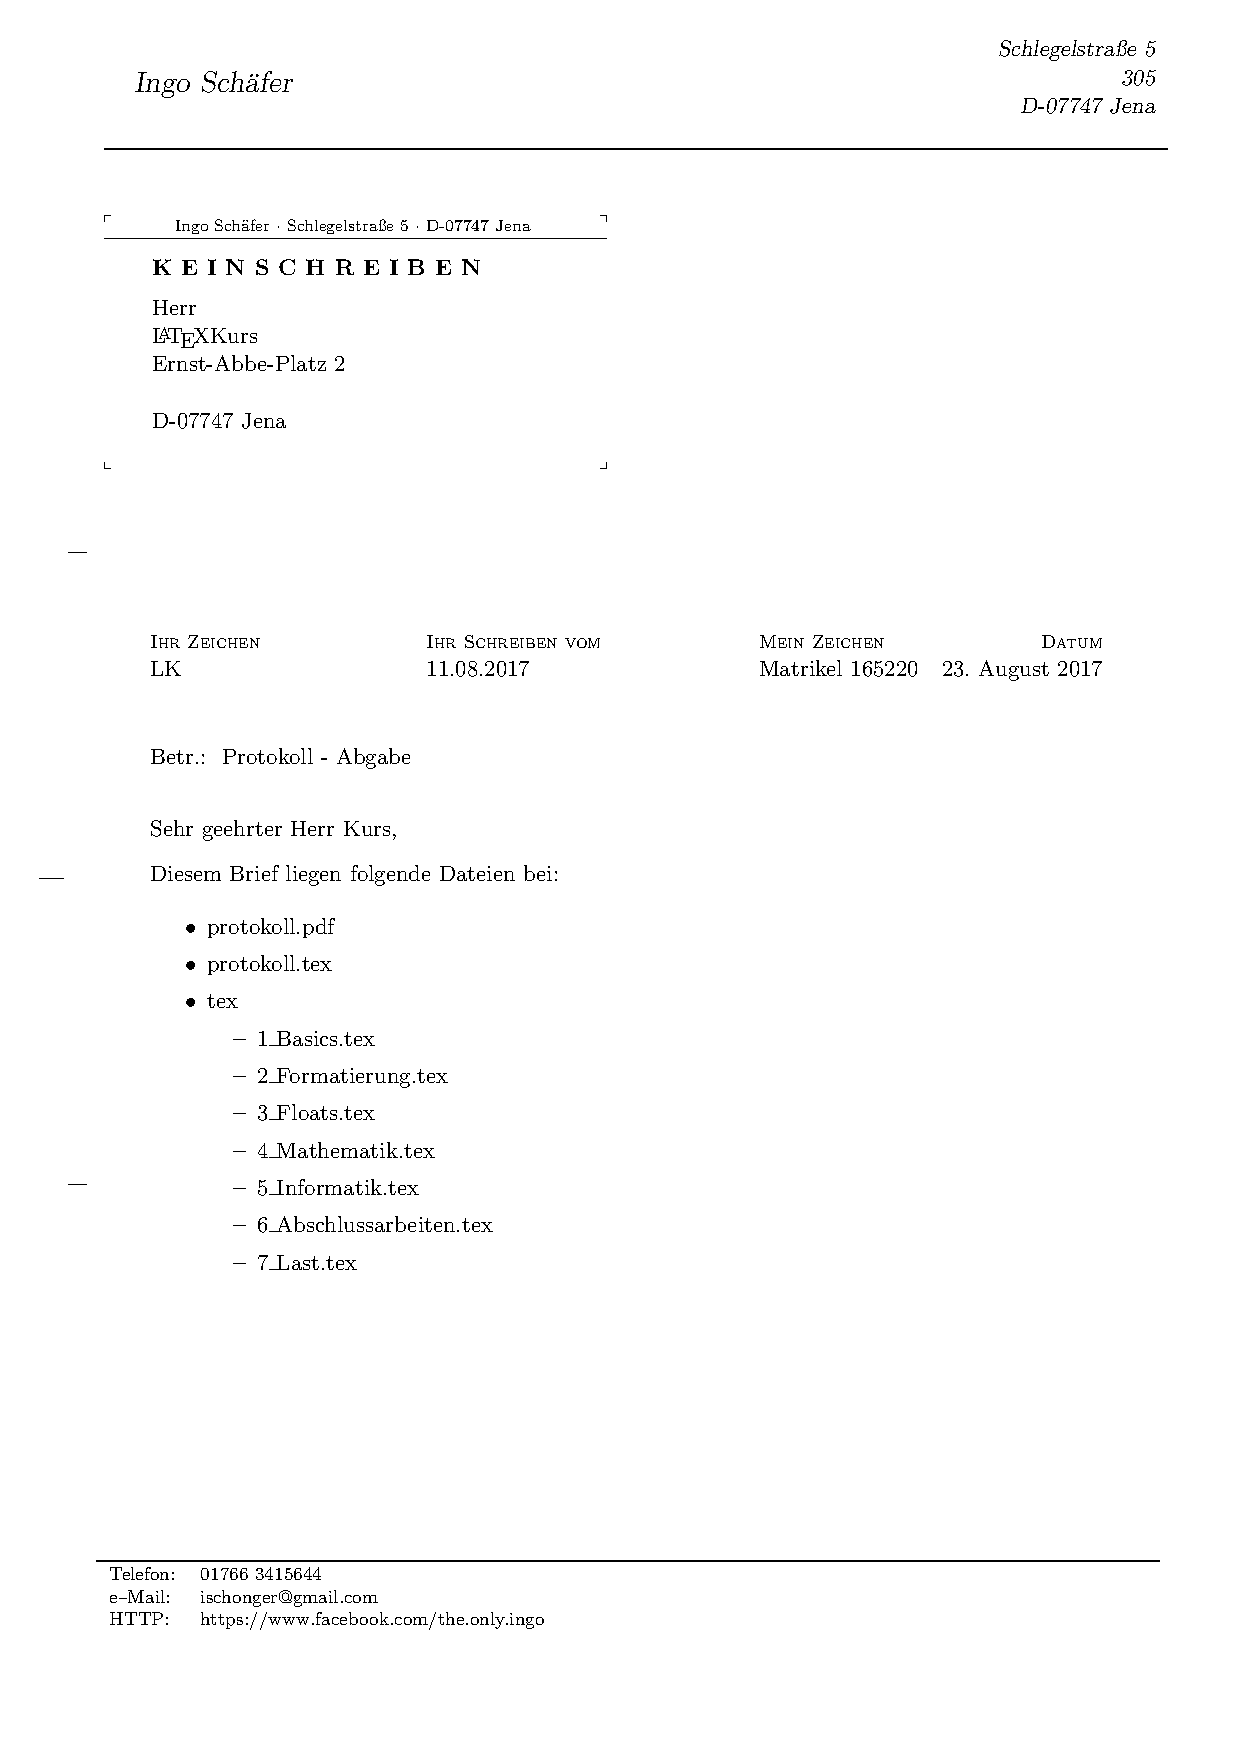
\includepdf[pages=1-3]{Aufgabe46/g-brief/beispiel.pdf}

%aufgabe 5
\maketitle

%aufgabe 6
\tableofcontents
\thispagestyle{empty}
%\setcounter{page}{0}		NOTE: Übersicht wird mitgezählt, aber nicht nummeriert.

% aufgabe 7
\pagebreak
\section*{Stärken und Schwächen von \LaTeX\ } 
\addcontentsline{toc}{section}{Stärken und Schwächen von \LaTeX\ }
\begin{quote}
\noindent
\LaTeX \ funktioniert nicht nach dem What-you-see-is-what-you-get - Prinzip.
Das mag erstmal etwas klobig in der Handhabung wirken, da immer wenn man seinen Schrieb anschauen will, das .tex-file
kompilieren muss.
Auch ist \LaTeX \ nicht in jedem Fall zu empfehlen: Eben bei solchen Arbeiten, wo man ständig nach dem Layout schauen muss
(z.B. Pixelschubsen bei Präsentationen, welche auch mit \LaTeX \ kreiert werden können), kann das ständige Zwischenkompilieren
nervig werden.
Besonders frickelig ist das Arbeiten mit Tabellen und Ähnlichem.
\LaTeX \ ist eher dafür gedacht ein bestimmtes Layout immer wieder verwenden zu können.
Darin liegt auch seine Stärke.
Oder auch das Vieles von \LaTeX \ automatisch gemacht wird. Wenn ich zum Beispiel eine Überschrift ändere, muss ich nicht in dem 
.tex-file nach weiteren Vorkommnissen (bspw. das Inhaltsverzeichnis suchen).
\LaTeX \ übernimmt sofort die Änderungen.
Besonders stark ist \LaTeX \ um wissenschaftliche Arbeiten zu Papier zu bringen.
Das Arbeiten mit Quellen, Fußnoten und Zitaten ist in \LaTeX \ super einfach gehalten.
Mathematische Formeln lassen sich auch sehr bequem aufschreiben.
Da \LaTeX \ alle möglichen Formelzeichen auf Halde hat, kommt man nicht in die Verlegenheit nur ähnliche Zeichen verwenden zu müssen.
Außerdem ist das Formelschreiben in \LaTeX \ wesentlich weniger frickelig als bspw. in Word.
\end{quote}


\pagebreak
\section{Basics}					% aufgabe 6
\label{sec:basics}
% aufgabe 7
\section*{Stärken und Schwächen von \LaTeX\ } 
\addcontentsline{toc}{section}{Stärken und Schwächen von \LaTeX\ }
\begin{quote}
\noindent
\LaTeX \ funktioniert nicht nach dem What-you-see-is-what-you-get - Prinzip.
Das mag erstmal etwas klobig in der Handhabung wirken, da immer wenn man seinen Schrieb anschauen will, das .tex-file
kompilieren muss.
Auch ist \LaTeX \ nicht in jedem Fall zu empfehlen: Eben bei solchen Arbeiten, wo man ständig nach dem Layout schauen muss
(z.B. Pixelschubsen bei Präsentationen, welche auch mit \LaTeX \ kreiert werden können), kann das ständige Zwischenkompilieren
nervig werden.
Besonders frickelig ist das Arbeiten mit Tabellen und Ähnlichem.
\LaTeX \ ist eher dafür gedacht ein bestimmtes Layout immer wieder verwenden zu können.
Darin liegt auch seine Stärke.
Oder auch das Vieles von \LaTeX \ automatisch gemacht wird. Wenn ich zum Beispiel eine Überschrift ändere, muss ich nicht in dem 
.tex-file nach weiteren Vorkommnissen (bspw. das Inhaltsverzeichnis suchen).
\LaTeX \ übernimmt sofort die Änderungen.
Besonders stark ist \LaTeX \ um wissenschaftliche Arbeiten zu Papier zu bringen.
Das Arbeiten mit Quellen, Fußnoten und Zitaten ist in \LaTeX \ super einfach gehalten.
Mathematische Formeln lassen sich auch sehr bequem aufschreiben.
Da \LaTeX \ alle möglichen Formelzeichen auf Halde hat, kommt man nicht in die Verlegenheit nur ähnliche Zeichen verwenden zu müssen.
Außerdem ist das Formelschreiben in \LaTeX \ wesentlich weniger frickelig als bspw. in Word.
\end{quote}
\pagebreak

% aufgabe 6
\subsection{Syntax}

\begin{aufgabe}
Richten Sie zun\"achst das \LaTeX\ Dokument ein. Nutzen Sie A4 Format,
hochkant, einspaltig, Schriftgr\"o\ss e 11\,pt.
\end{aufgabe}	


\begin{aufgabe}
Setzen Sie die Seitenr\"ander auf 3\,cm (oben, rechts, links) und 3,5\,cm
(unten).
\end{aufgabe}

\subsection{Erzeugen des Dokuments}
\begin{aufgabe}
Passen Sie Kopf- und Fu\ss zeilen des Dokuments folgenderma\ss en an:
Kopfzeile links enth\"alt Ihren Namen, Kopfzeile rechts Ihre Matrikelnummer;
Fu\ss{}zeile mitte enth\"alt die Seitenzahl in der Form ``x von X''.
\end{aufgabe}


\begin{aufgabe}
F\"ugen Sie nach diesem Abschnitt einen Seitenumbruch ein.	
\end{aufgabe}

%aufgabe 4
\pagebreak % oder \clearpage


\subsection{Dokumentaufbau, Seitenlayout und Präambel}
\begin{aufgabe}
F\"ugen Sie dem Dokument einen Titel f\"ur das Protokoll, Datum sowie Ihren
eigenen Namen und Matrikelnummer als Autor hinzu. Die Titelseite soll auf
einer einzelnen Seite erscheinen.
\end{aufgabe}	

\subsection{Dokumentsruktur}
\begin{aufgabe}
Gliedern Sie das Protokoll in einzelne Abschnitte entsprechend des Ablaufs
des Seminars. F\"ugen Sie ein Inhaltsverzeichnis ein. Das Inhaltsverzeichnis
soll auf einer einzelnen Seite stehen.
\end{aufgabe}

\begin{aufgabe}
F\"ugen Sie einen \textbf{unnummerierte} Abschnitt (z.B.\ ``Was ist
\LaTeX?'') an den Anfang des Protokolls, in der Sie eine kurze (ca.\ 150
W\"orter) Zusammenfassung zu \LaTeX\ schreiben. Der Abschnitt soll im
Inhaltsverzeichnis auftauchen.
\end{aufgabe}

\begin{multicols}{2}
\begin{aufgabe}
Setzen Sie diese Aufgabe in ein zweispaltiges Format. Der horizontale Abstand zwischen den Spalten soll 1\,cm betragen. Die beiden Spalten sollen durch eine 2\,pt dicke vertikale Linie getrennt werden. 		
\end{aufgabe}
\end{multicols}


\subsection{Crossreferencing}
\label{subs:Crossreferencing}
\begin{aufgabe}
\label{aufg:9}
F\"ullen Sie in folgendem Satz die mit \textbf{XX} gekennzeichneten Stellen
mittels Crossreferencing.
\end{aufgabe}
In Aufgabe~\mycommand{aufg:9} im Abschnitt~\mycommand{subs:Crossreferencing} auf Seite~\textbf{\pageref{subs:Crossreferencing}}
behandeln wir die Verwendung von Labels um unkompliziert innerhalb des
Dokuments zu referenzieren.


\pagebreak
\section{Textformatierung}				% aufgabe 6
\label{sec:textformatierung}
\subsection{Encoding}
\begin{aufgabe}
Verwenden Sie das richtige Input und Output Encoding und setzen Sie die Spracheinstellungen auf die neue deutsche Rechtschreibung.	
\end{aufgabe}

\begin{aufgabe}
\TeX en Sie folgenden Text so exakt wie m\"oglich nach.	
\end{aufgabe}
\noindent \underline{Ursprungstext:} \\
\noindent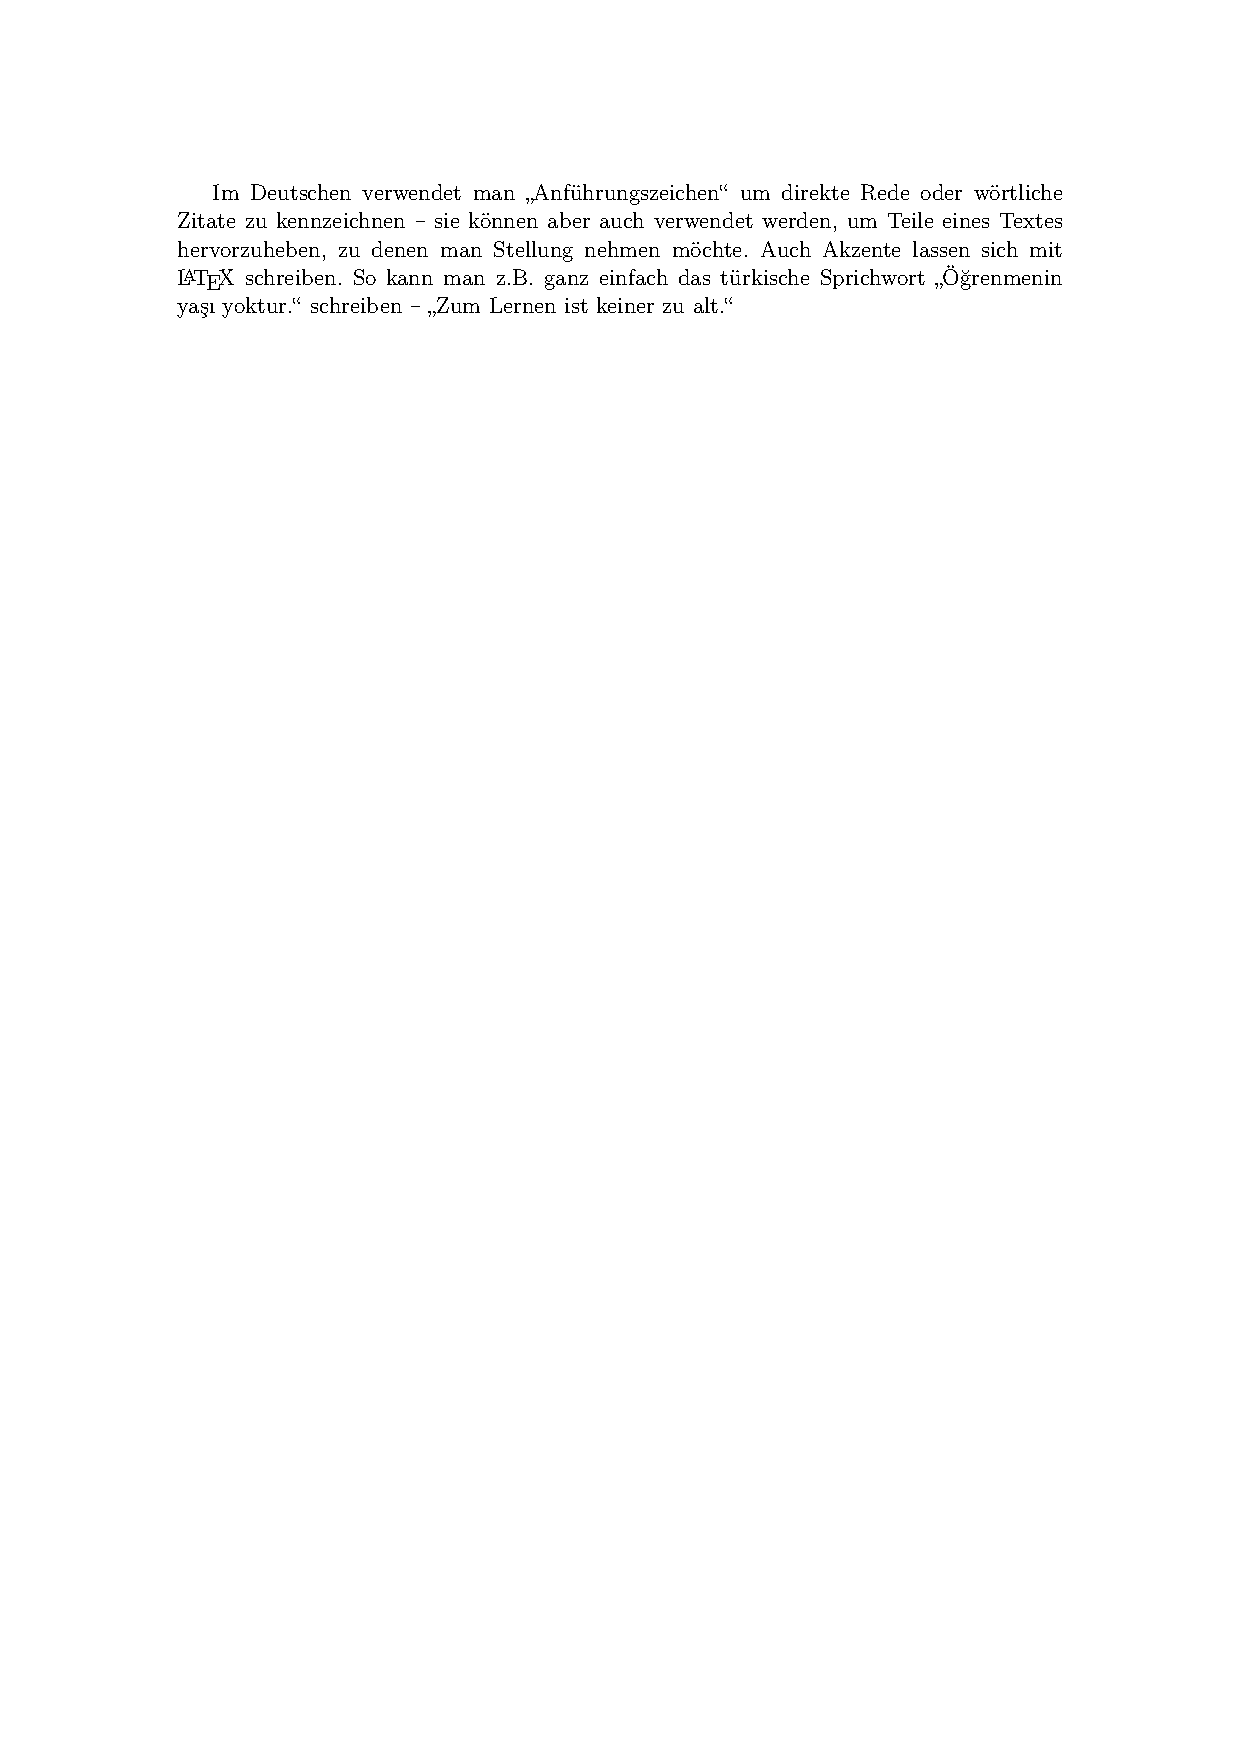
\includegraphics[width=\textwidth]{aufgabe11}

\noindent \underline{nachge\TeX t:}\\
\singlespacing
\indent Im Deutschen verwendet man \glqq Anführungszeichen\grqq \ um direkte Rede oder wörtliche Zitate zu kennzeichnen -- 
sie können aber auch verwendet werden, um Teile eines Textes hervorzuheben, zu denen man Stellung nehmen möchte.
Auch Akzente lassen sich mit \LaTeX\ schreiben.
So kann man z.B. ganz einfach das türkische Sprichwort \glqq Ö\u{g}renmenin ya\c{s}{\i} yoktur.\grqq \ schreiben  -- 
\glqq Zum Lernen ist keiner zu alt.\grqq

\subsection{Schriften}					% aufgabe 6
\begin{aufgabe}
\TeX en Sie folgenden Text so exakt wie m\"oglich nach.	
\end{aufgabe}

\noindent \underline{Ursprungstext:} \\
\noindent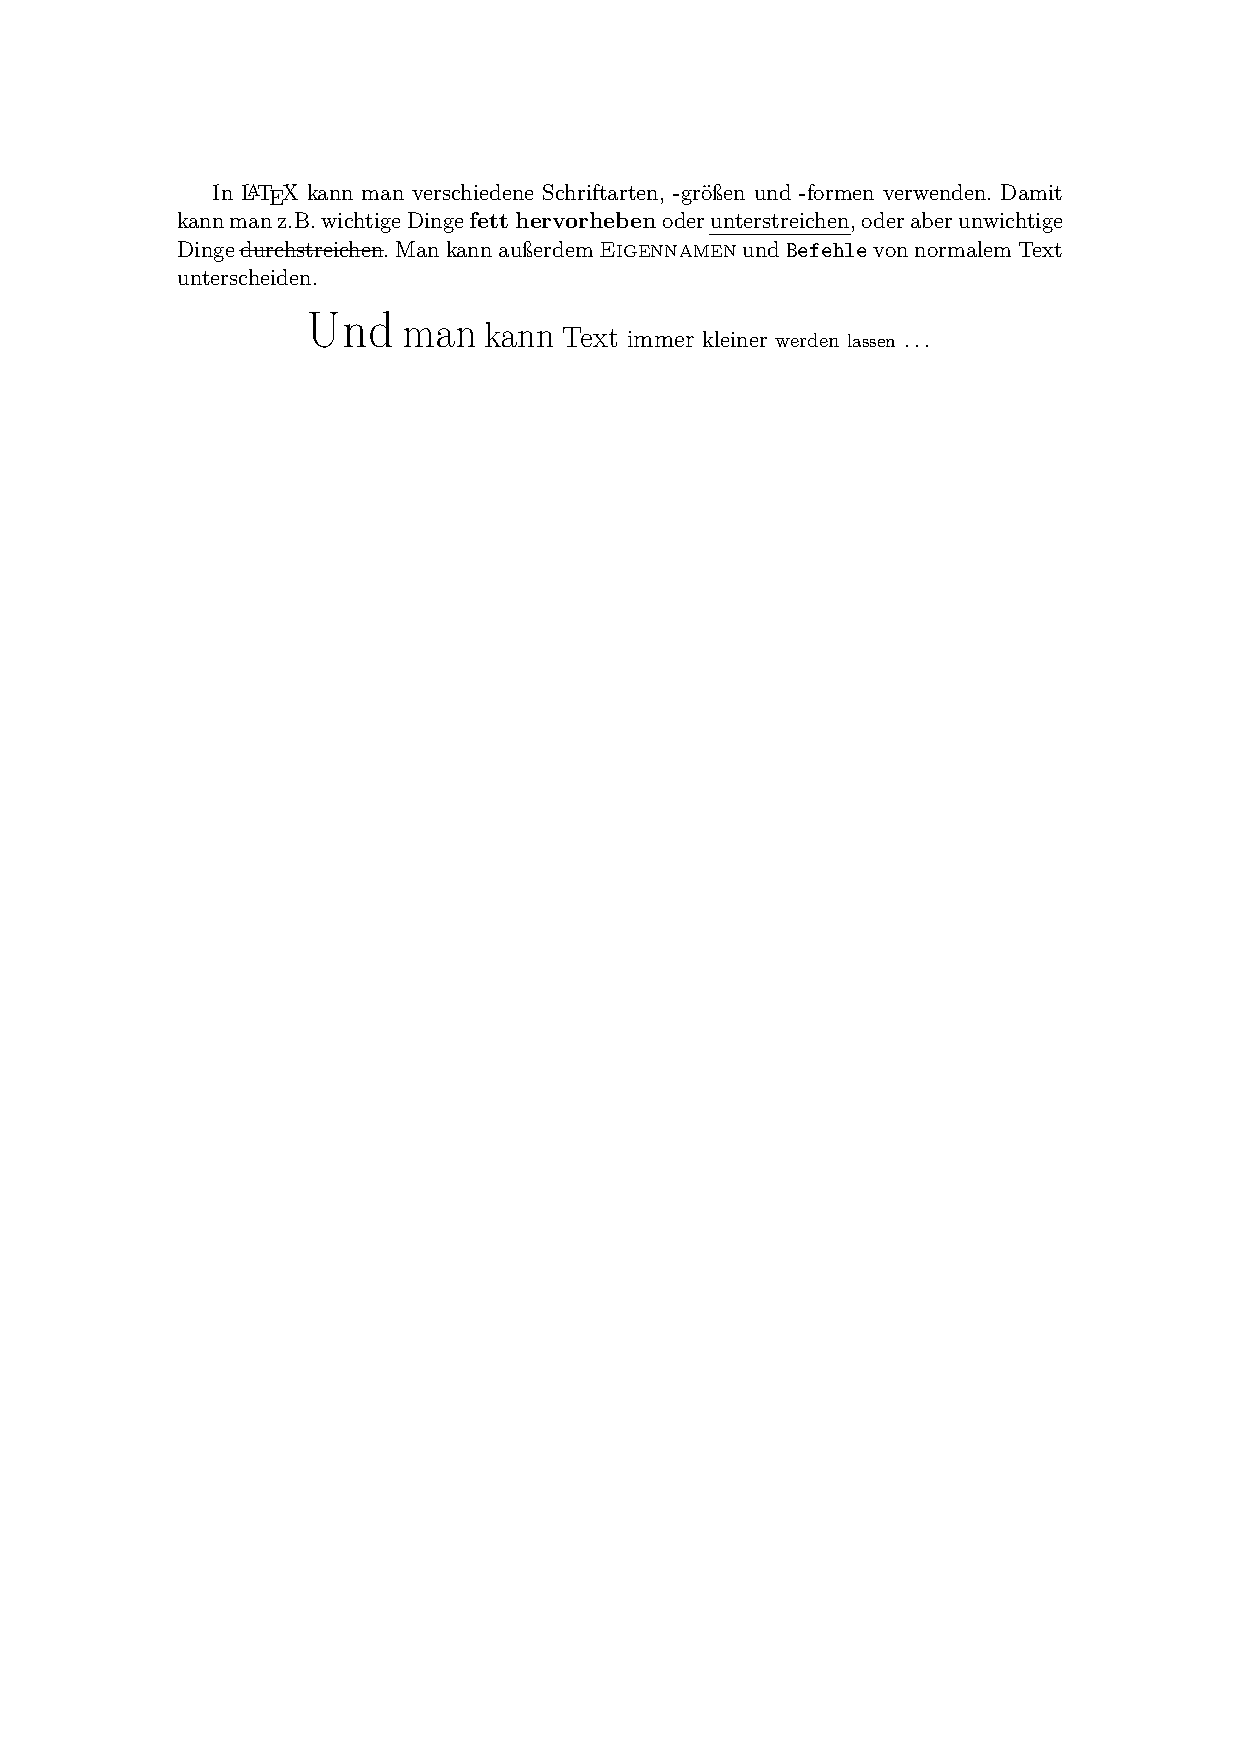
\includegraphics[width=\textwidth]{aufgabe12}

\noindent \underline{nachge\TeX t:}\\
\indent 
In \LaTeX\ kann man verschiedene Schriftarten, -größen und -formen verwenden.
Damit kann man z.B.\ wichtige Dinge \textbf{fett hervorheben} oder \underline{unterstreichen}, oder aber unwichtige Dinge
\sout{durchstreichen}.
Man kann außerdem \textsc{Eigennamen} und \texttt{Befehle} von normalem Text unterscheiden.
\\
\\
\noindent\hspace*{21mm}
\Huge{Und} \huge{man} \LARGE{kann} \Large{Text} \large{immer} \normalsize{kleiner} \small{werden} \footnotesize{lassen}
\dots

\pagebreak
\subsection{White Space}				% aufgabe 6
\normalsize
\begin{aufgabe}
\TeX en Sie folgenden Text so exakt wie m\"oglich nach.	
\end{aufgabe}

\noindent \underline{Ursprungstext:} \\
\noindent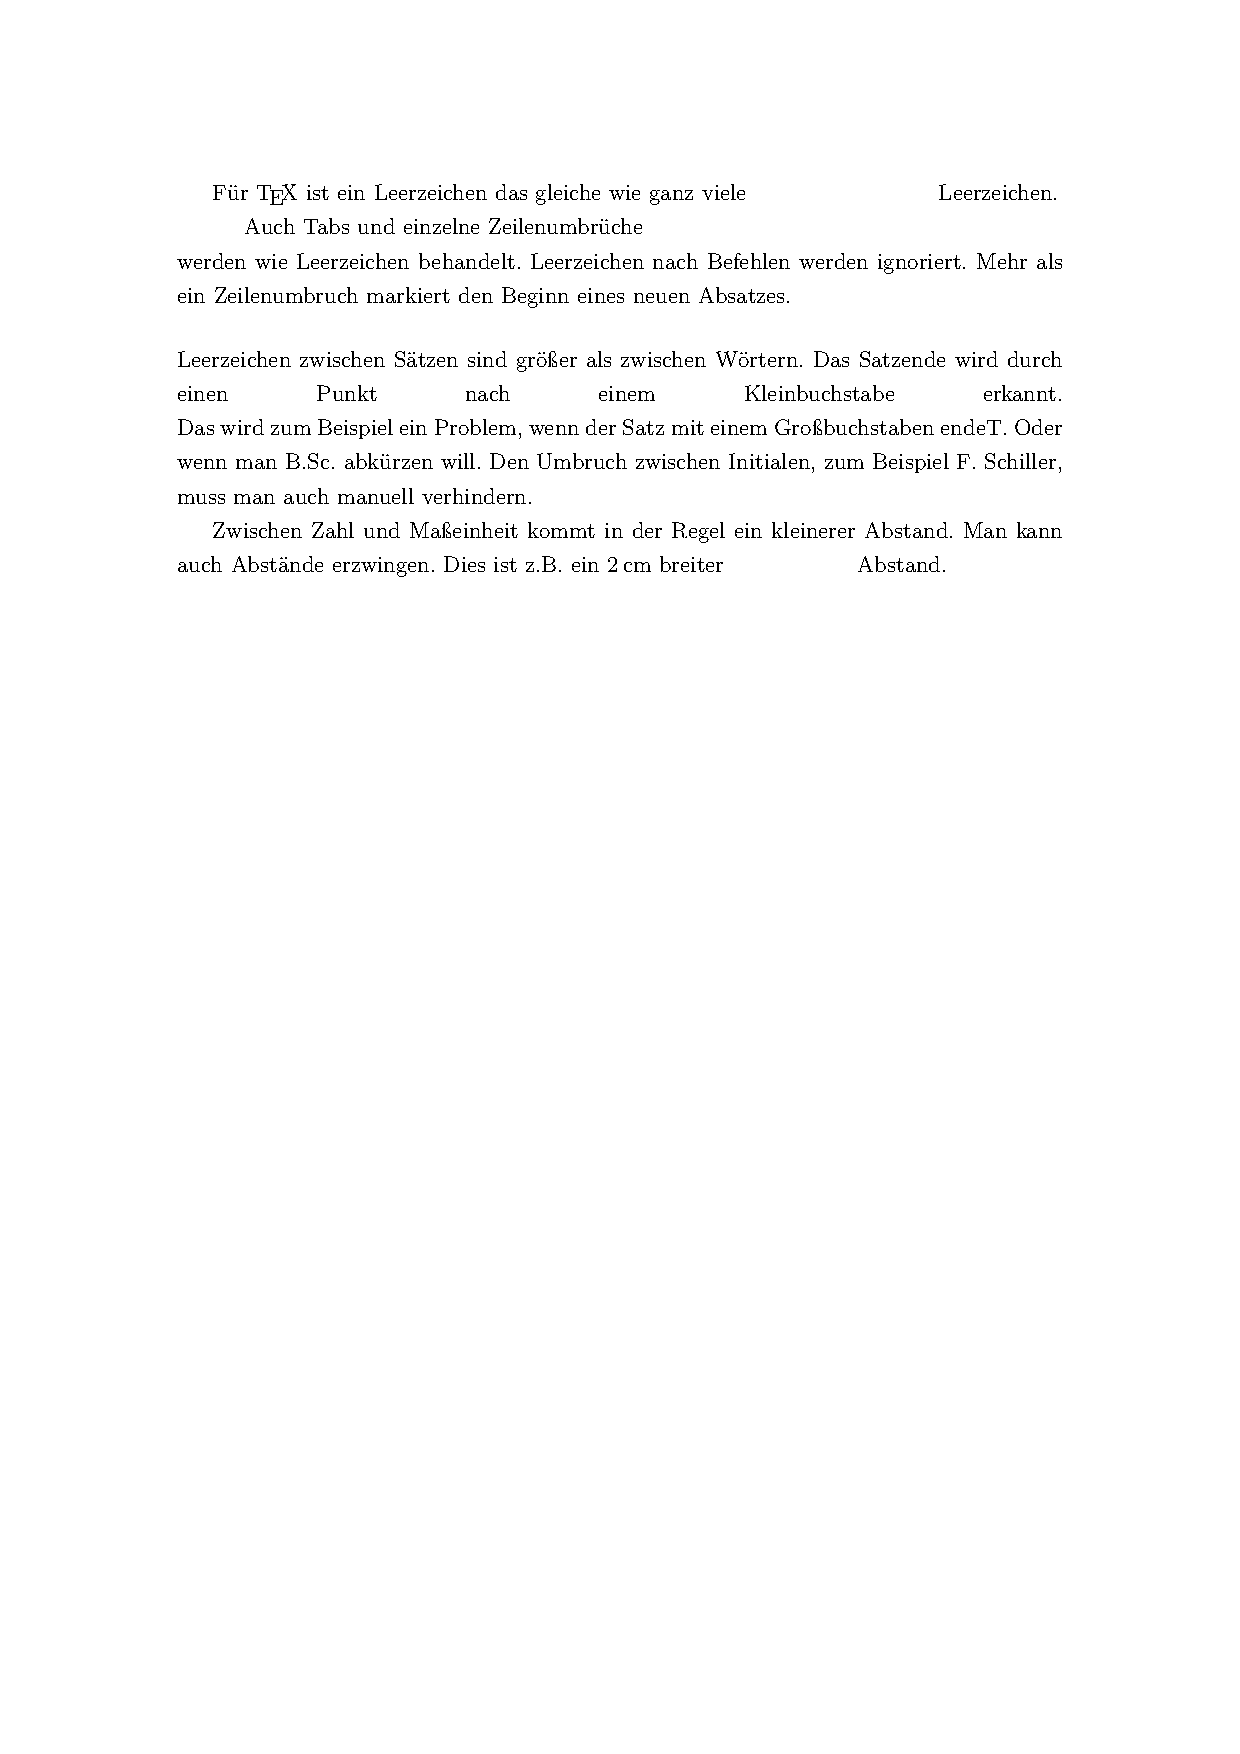
\includegraphics[width=\textwidth]{aufgabe13}

\noindent \underline{nachge\TeX t:}\\
\normalsize
%\begin{onehalfspacing}
\onehalfspacing
\indent Für \TeX \ ist ein Leerzeichen das gleiche wie ganz viele \hfill Leerzeichen.\\
\setlength{\parindent}{12mm} \indent 
Auch Tabs und einzelne Zeilenumbrüche\\
werden wie Leerzeichen behandelt. Leerzeichen nach Befehlen werden ignoriert.
Mehr als ein Zeilenumbruch markiert den Beginn eines neuen Absatzes.\\
\\
Leerzeichen zwischen Sätzen sind größer als zwischen Wörtern. Das Satzende wird durch\\
einen Punkt nach einem Kleinbuchstabe erkannt.\linebreak
Das wird zum Beispiel ein Problem, wenn der Satz mit einem Großbuchstaben endeT.\
Oder wenn man B.Sc.\ abkürzen will.
Den Umbruch zwischen Initialen, zum Beispiel F.~Schiller, muss man auch manuell verhindern.\\
\hspace*{4mm} Zwischen Zahl und Maßeinheit kommt in der Regel ein kleinerer Abstand.
Man kann auch Abstände erzwingen.
Dies ist z.B. ein 2cm breiter \hspace{2cm} Abstand.
%\end{onehalfspacing}

\pagebreak
\subsection{Listen}					% aufgabe 6
\begin{aufgabe}
\TeX en Sie folgenden Text so exakt wie m\"oglich nach.	
\end{aufgabe}

\noindent \underline{Ursprungstext:} \\
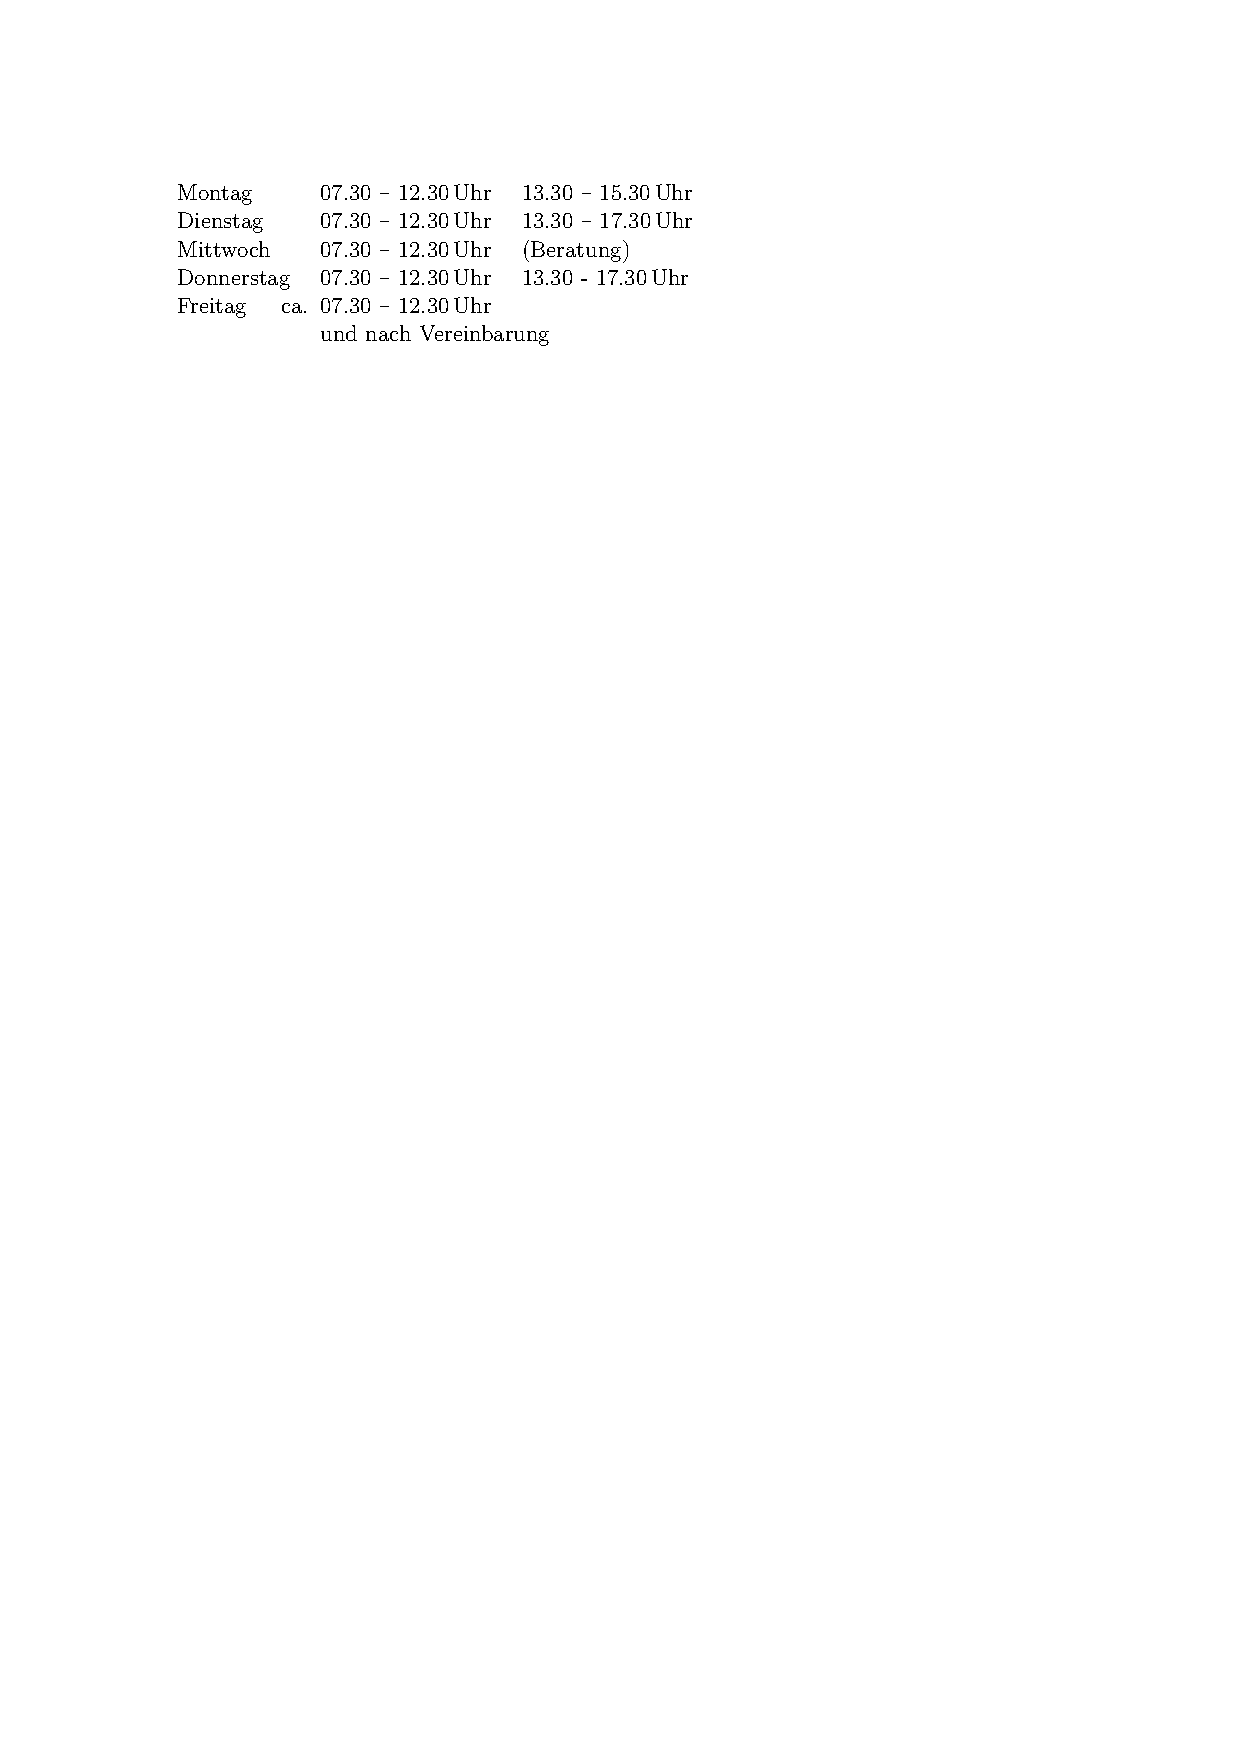
\includegraphics[width=\textwidth]{aufgabe14}

\noindent \underline{nachge\TeX t:}\\
\begin{singlespacing}
\hspace{-1.45cm}
\begin{tabular}{l l l}
Montag 		& 07.30 – 12.30 Uhr & \hspace{-0.9cm} 13.30 – 15.30 Uhr \\
Dienstag 	& 07.30 – 12.30 Uhr & \hspace{-0.9cm} 13.30 – 17.30 Uhr \\
Mittwoch 	& 07.30 – 12.30 Uhr & \hspace{-0.9cm} (Beratung) \\
Donnerstag 	& 07.30 – 12.30 Uhr & \hspace{-0.9cm} 13.30 – 17.30 Uhr \\
Freitag 	& \hspace{-0.74cm} ca. 07.30 – 12.30 Uhr &  \\
& und nach Vereinbarung & \\
\end{tabular}
\end{singlespacing}

\pagebreak
\begin{aufgabe}
Erstellen Sie folgende Liste.
\end{aufgabe}

\noindent \underline{Ursprungstext:} \\
\noindent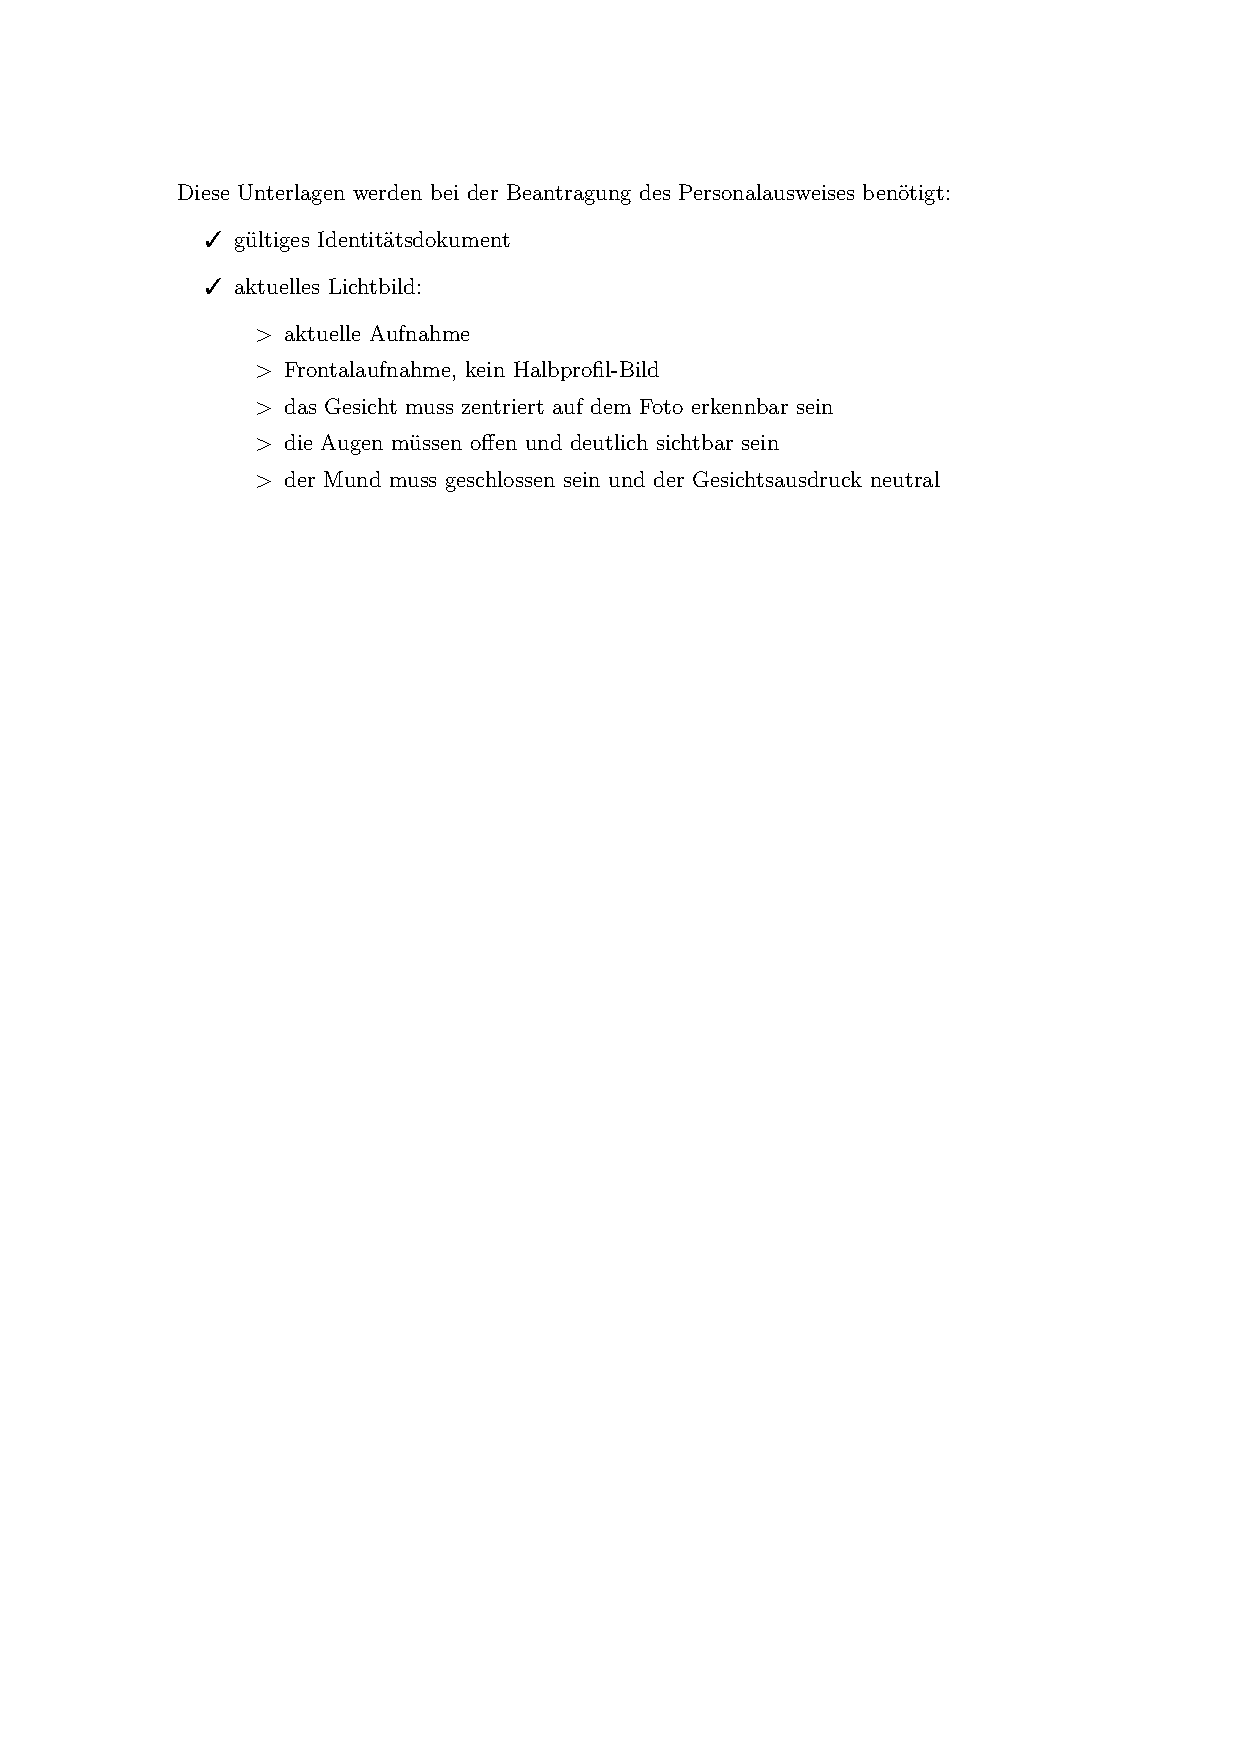
\includegraphics[width=\textwidth]{aufgabe15}

\noindent \underline{nachge\TeX t:}\\
Diese Unterlagen werden bei der Beantragung des Personalausweises benötigt:

\begin{itemize}
 \item[\ding{51}] gültiges Indentitätsbild
 \item[\ding{51}] aktuelles Lichtbild:
  \begin{itemize}
   \item[>] aktuelle Aufnahme
   \item[>] Frontalaufnahme, kein Halbprofil-Bild
   \item[>] das Gesicht muss zentriert auf dem Foto erkennbar sein
   \item[>] die Augen müssen offen und deutlich sichtbar sein
   \item[>] der Mund muss geschlossen sein und der Gesichtsausdruck neutral
  \end{itemize}
\end{itemize}


\begin{aufgabe}
Generieren Sie eine 1\,cm einger\"uckte Liste, die mit (A1), (A2), (A3),\dots\ gelabelt ist. Schreiben Sie darunter einen Satz, der auf das erste Element der Liste verweist.
\end{aufgabe}

\begin{enumerate}[\hspace{1cm} ({A}1)]
 \item Hund \label{it:hund}
 \item Katze \label{it:katze}
 \item Maus
 \item Marder
 \item Dachs
 \item Bieber
\end{enumerate}

\noindent Der Hund (A\ref{it:hund}) ist ein Haustier, das Geruch erzeugt.

\pagebreak
\begin{aufgabe}\label{aufg:desc}
Erstellen Sie eine \textnormal{\texttt{description}} Liste, in der Sie kurz
(je ein Satz) \TeX, \LaTeX\ und Word (im Hinblick auf deren Unterschiede)
beschreiben.
\end{aufgabe}

\begin{description}
 \item[\TeX] TeX ist ein Textsatzsystem mit eingebauter Makrosprache.
 \item[\LaTeX] LaTeX ist ist ein Softwarepaket, das die Benutzung des Textsatzsystems \TeX mit Hilfe von Makros vereinfacht.
 \item[Word] Word von Microsoft ist ein WYSIWYG-Editor.
\end{description}

\subsection{Fußnoten}						% aufgabe 6
\begin{aufgabe}
\label{aufg:18}
\setcounter{footnote}{2}
\renewcommand{\thefootnote}{\fnsymbol{footnote}}
F\"ugen Sie dieser Aufgabe eine Fu\ss note hinzu. Die Fu\ss{}note soll mit dem dritten Fu\ss{}notensymbol
gekennzeichnet sein. Sie soll mindestens 1\,cm  vom Haupttext entfernt mittels einer gepunkteten Linie 
abgetrennt werden.\footnote{Dies ist die Fußnote für Aufgabe \ref{aufg:18}.}
\end{aufgabe}

Vielleicht sollte aber auch die dritte Nummerierung benutzt werden. 
Schließlich steht ja nirgendwo festgeschrieben, 
dass~\verb*|\ddagger| das dritte Symbol ist. 
\hspace{-0.1cm}\footnote[3]{Dann ist das hier eine andere Fußnote für Aufgabe \ref{aufg:18}.}

\subsection{Randnotizen}
\begin{aufgabe}
Nutzen Sie Randnotizen um diese Aufgabe links mit einem 3\,mm breiten und 8\,mm hohen Balken zu markieren.

\reversemarginpar
\marginpar{\rule[0pt]{3mm}{8mm}}
\end{aufgabe}

\subsection{Boxen und Silbentrennung}
\begin{aufgabe}
\TeX en Sie folgende 3\,cm breite eingerahmte Box so exakt wie m\"oglich nach und achten Sie dabei insbesondere auf die korrekte Silbentrennung.
\end{aufgabe}

\noindent \underline{Ursprung:} \\
\noindent
\includegraphics[width=\textwidth]{aufgabe20}

\noindent \underline{nachge\TeX t:}\\
\indent \hspace{-0.7cm}
\fbox{\begin{minipage}{3cm}
  \begin{onehalfspacing}
   Gas\-chro\-ma\-to\-gra-\ \\phie\--Mass\-enspek-\ \\tro\-me\-trie
  \end{onehalfspacing}
\end{minipage}}

\subsection{Farben}						% aufgabe 6
\begin{aufgabe}
\"Andern Sie die Hintergrundfarbe nur dieser Seite in einen sehr hellen Pastellton (mindestens 90\,\% Wei\ss{}anteil). (Der Einfachheit halber k\"onnen Sie den n\"achsten Abschnitt auf einer neuen Seite beginnen.)
\end{aufgabe}
\pagecolor{LightGrey}

\pagebreak
\section{Abbildungen und Tabellen}			% aufgabe 6
\label{sec:floats}
\subsection{Abbildungen}
\pagecolor{white}
\begin{aufgabe}\label{aufg:fig} \label{aufg:22}
F\"ugen Sie ein beliebiges Bild ein, das 10\,cm breit ist und oben und unten um 1cm zurecht geschnitten wurde. 
\end{aufgabe}

\afterpage{
\begin{figure}[t] 		% aufgabe 24
\centering 			% aufgabe 24
\setlength{\fboxrule}{1pt} 	% aufgabe 23
% aufgabe 21
\fbox{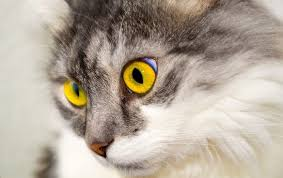
\includegraphics[width=10cm,clip=true,trim= 0cm 1cm 0cm 1cm]{cat.jpg}} 
\caption[Die Katzen (Felidae)]
	{Dies ist eine süße kleine Katze im Miniformat. Aaaaawww\dots\\		% aufgabe 24
	\glqq Die Katzen (Felidae) sind eine Familie aus der Ordnung der Raubtiere (Carnivora) innerhalb der Überfamilie
	der Katzenartigen (Feloidea). Sie sind auf allen Kontinenten außer Ozeanien und Antarktika verbreitet und 
	nahezu ausschließlich Fleischfresser. Eingeteilt werden sie in Großkatzen (wie beispielsweise Löwe, Tiger 
	und Leopard) und Kleinkatzen (etwa Wildkatze, Luchs und Ozelot), wobei zu den Kleinkatzen auch große
	Vertreter wie der Puma und – nach neueren molekulargenetischen Erkenntnissen – der Gepard gehören. 
	Mit der von der Wildkatze abstammenden Hauskatze wurde ein Vertreter der Familie durch Domestizierung 
	zu einem Begleiter des Menschen.\grqq \\ (aus https://de.wikipedia.org/wiki/Katzen, 23.08.2017)}	
\label{abb:cat} 		% aufgabe 24
\end{figure}}

\begin{aufgabe}
\label{aufg:23}
Legen Sie das Bild aus der vorherigen Aufgabe in ein eigenes Verzeichnis f\"ur Abbildungen. \"Ubergeben Sie \LaTeX\ das Abbildungsverzeichnis global.	
\end{aufgabe}

\begin{aufgabe}
\label{aufg:24}
Rahmen Sie die Abbildung aus Aufgabe~\ref{aufg:fig} mit einem 1\,pt dicken Rahmen ein.
\end{aufgabe}

\begin{aufgabe}
\label{aufg:25}
Setzen Sie die Abbildung aus Aufgabe~\ref{aufg:fig} in eine Float Umgebung und f\"ugen Sie ihr eine geeignete Bildunterschrift hinzu, welche \"uber mehrere Zeilen reicht. Die Abbildung soll sich am oberen Seitenrand befinden und zentriert sein. Schreiben Sie unter diese Aufgabe einen Satz, in dem Sie auf die Abbildung verweisen.	
\end{aufgabe}
\FloatBarrier			% aufgabe 30
In der Bildunterschrift der Abbildung \ref{abb:cat} wird der Einleitungstext aus dem Wikipedia-Artikel über Katzen zitiert.

\pagebreak
\begin{aufgabe}
F\"ugen Sie eine weitere Abbildung in einer weiteren  Float Umgebung ein. 
Die Abbildung soll 14\,cm hoch sein, aber nicht \"uber den Seitenrand hinaus gehen. 
Die Abbildung soll eine geeignete mehrzeilige Bildunterschrift erhalten. 
Die Abbildung soll sich \textsc{nicht} auf einer einzelnen Seite befinden.
\end{aufgabe}

\FloatBarrier
\begin{figure}[h]
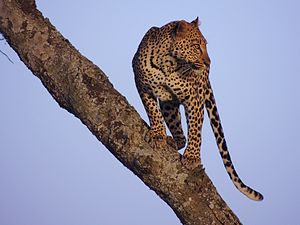
\includegraphics[height=14cm, width=\textwidth, keepaspectratio=false]{leo}
\caption[Der Leopard (Panthera pardus)]
	{Der Leopard (Panthera pardus) ist eine Art aus der Familie der Katzen, die in Afrika und Asien verbreitet ist.}
\end{figure}
\FloatBarrier


\begin{aufgabe}
F\"ugen Sie dem Protokoll ein Abbildungsverzeichnis hinzu. Die Bildunterschriften im Abbildungsverzeichnis sollen nicht \"uber eine Zeile hinaus gehen.
\end{aufgabe}

\pagebreak
\begin{aufgabe}
F\"ugen Sie zwei Abbildungen (Bannerformat) untereinander ein. 
Die Abbildungen sollen jeweils eine eigene und eine gemeinsame Bildunterschrift erhalten. 
Verweisen sie auf eine der beiden Teilabbildungen.

\begin{figure}[h]
 \begin{subfigure}[h]{\textwidth}
  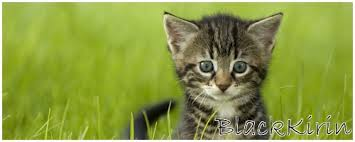
\includegraphics[width=\textwidth]{ban1.jpg}
  \caption{Das ist die erste Banner Katze.}
  \label{abb:banner1}
 \end{subfigure}
 
 \begin{subfigure}[h]{\textwidth}
  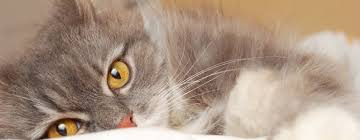
\includegraphics[width=\textwidth]{ban2.jpg}
    \caption{Das ist die zweite Banner Katze.}
 \end{subfigure}
  
 \caption{Diese Abbildung verdeutlicht den Vorteil von Subfigure~-~Umgebungen.}
\end{figure}
\end{aufgabe}
\FloatBarrier
Besonders katzig ist die Bannerkatze aus Abbildung \ref{abb:banner1}.

\pagebreak
\begin{aufgabe}
F\"ugen Sie zwei Abbildungen nebeneinander ein. Die Abbildungen sollen die gleiche H\"ohe haben und jeweils eine eigene und eine gemeinsame Bildunterschrift erhalten.

\begin{figure}
 \centering
 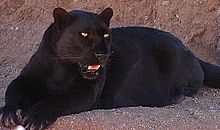
\includegraphics[height=3cm]{blacky}
 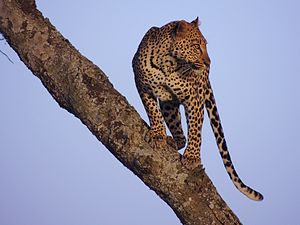
\includegraphics[height=3cm]{leo}
\caption{Diese beiden Tiere gehören derselben Art Katze an.}
\label{img:nebeneinander}
\end{figure}
\end{aufgabe}
\noindent (Abbildung \ref{img:nebeneinander} oberhalb der Aufgabenstellung.)


\begin{aufgabe}
Verwenden Sie einen geeigneten Befehl, damit keine der Abbildungen nach der n\"achsten Aufgabe erscheint.
\end{aufgabe}
Da die Aufgaben \ref{aufg:22}, \ref{aufg:23}, \ref{aufg:24}, \ref{aufg:25} sich alle auf ein Bild (Abbildung \ref{abb:cat}) beziehen,
habe ich dieses Bild auf die nächste Seite gelegt.
Dadurch wird auch das Design nicht zerstückelt.
Ich wollte, dass die Kapitelüberschrift von Kapitel \ref{sec:floats} auf einer neuen Seite (Seite \pageref{abb:cat}) steht.
Wäre zuerst das Bild gekommen, wäre das uneinheitlich gegenüber dem Gesamtaussehen des Protokolls gewesen.

\pagebreak
\subsection{Tabellen}
\begin{aufgabe}
\TeX en Sie folgende Tabelle so exakt wie m\"oglich nach.	
\end{aufgabe}

\noindent \underline{Ursprung:} \\
\noindent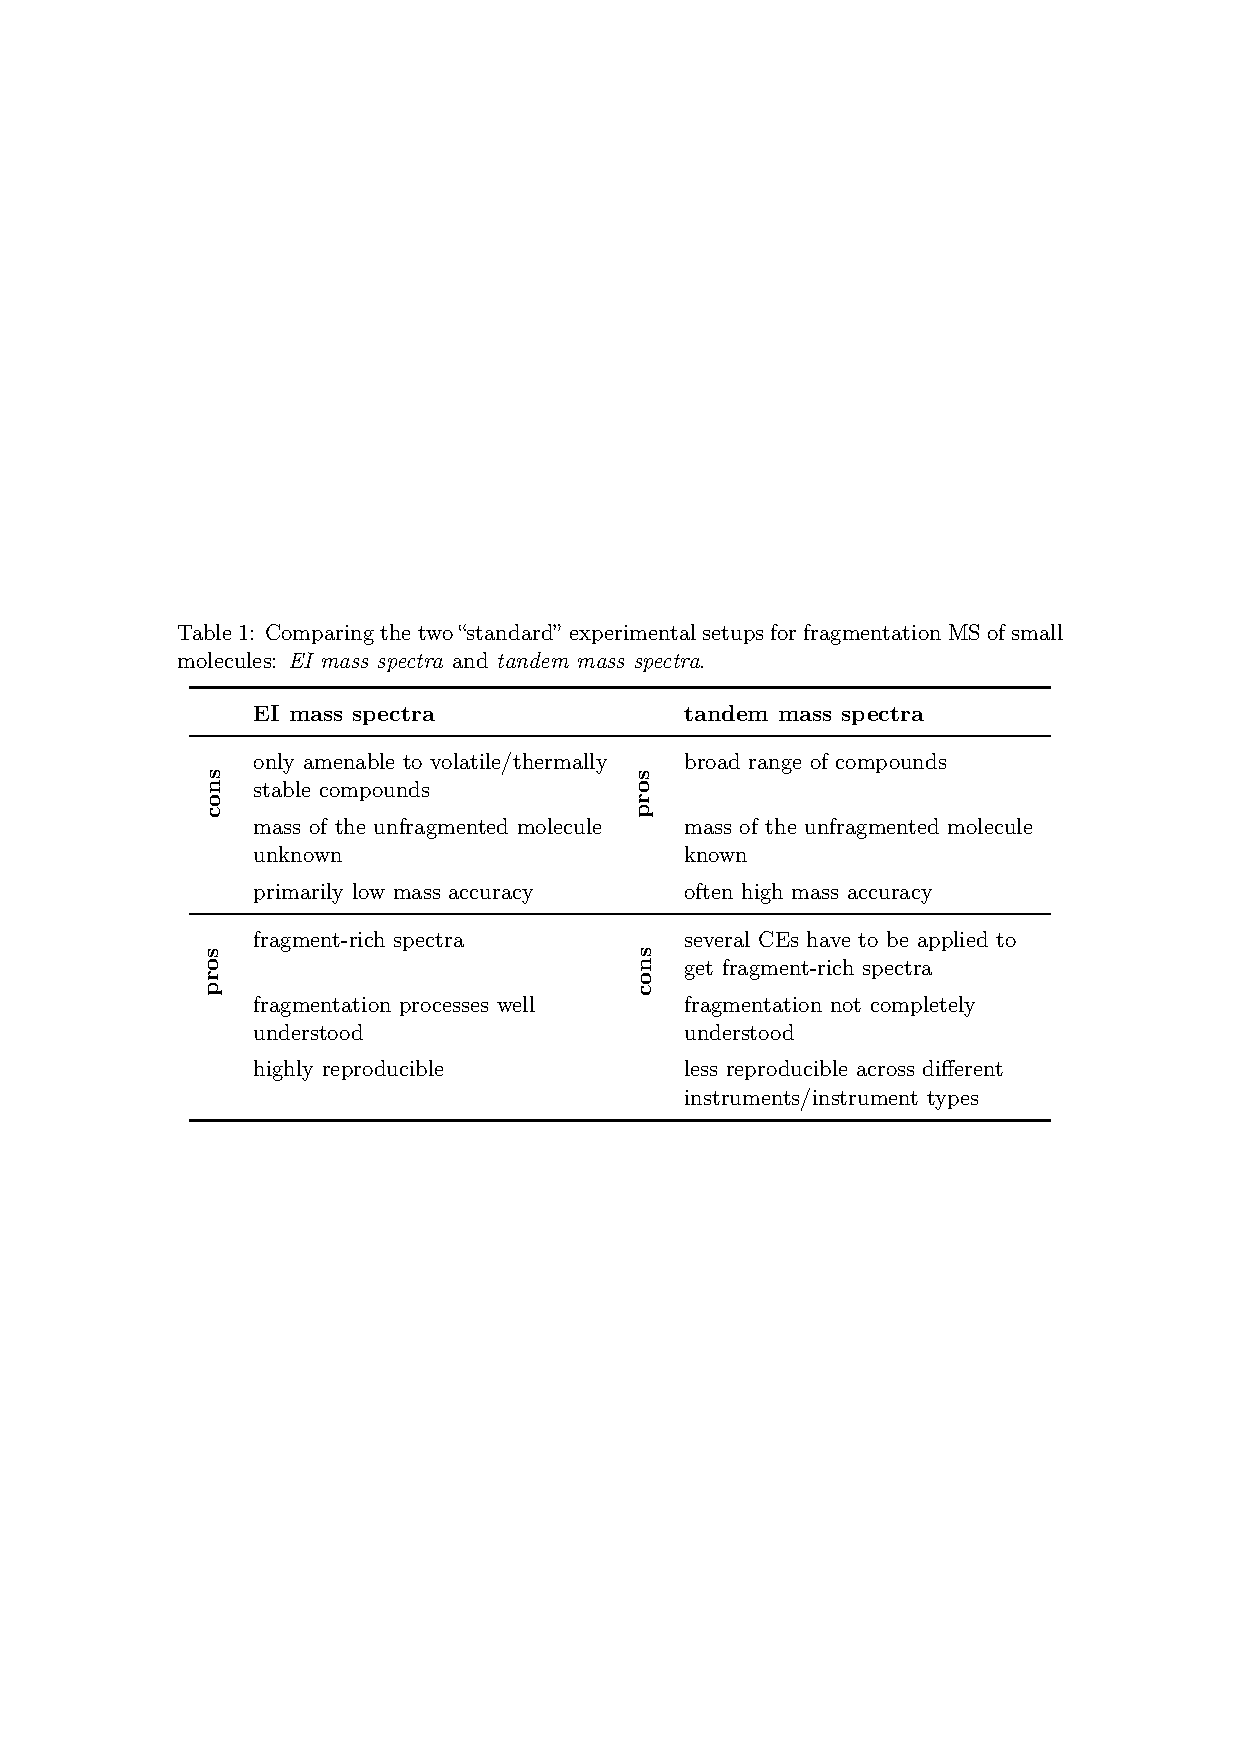
\includegraphics[width=\textwidth]{aufgabe31}

\noindent \underline{nachge\TeX t:}\\
\FloatBarrier
\begin{table}[H]
\selectlanguage{english}
 \caption[Comparing the two “standard” experimental setups for fragmentation MS]
	 {Comparing the two “standard” experimental setups for fragmentation MS of small
	  molecules: \textit{EI mass spectra} and \textit{tandem mass spectra}.\\
	  }
	  \vspace{-0.6cm} \hspace{2mm}
\begin{tabularx}{\textwidth}{p{0.04\textwidth} p{0.4\textwidth} p{0.04\textwidth} p{0.4\textwidth}}
 \toprule
 & \textbf{EI mass spectra} &  & \textbf{tandem mass spectra} \\
 \midrule
    \multirow{3}*{\begin{sideways} \textbf{cons} \end{sideways}}
  & only amenable to volatile/thermally
    stable compounds\newline
    mass of the unfragmented molecule
    unknown\newline
    primarily low mass accuracy\newline
  & \multirow{3}*{\begin{sideways} \textbf{pros} \end{sideways}}  
  & broad range of compounds\newline \newline
    mass of the unfragmented molecule
    known\newline
    often high mass accuracy\\
    \midrule
    \multirow{3}*{\begin{sideways} \textbf{pros} \end{sideways}}
  & fragment-rich spectra\newline
    \newline
    \raggedright{ processes well
    understood}\newline
    highly reproducible
  & \multirow{3}*{\begin{sideways} \textbf{cons} \end{sideways}}
  & several CEs have to be applied to
    get fragment-rich spectra\newline
    fragmentation not completely
    understood\newline
    less reproducible across different
    instruments/instrument types\\
 \bottomrule
\end{tabularx}
\end{table}

\pagebreak
\begin{aufgabe}
\TeX en Sie folgende Tabelle so exakt wie m\"oglich nach.		
\end{aufgabe}
\FloatBarrier
\noindent \underline{Ursprung:} \\
\noindent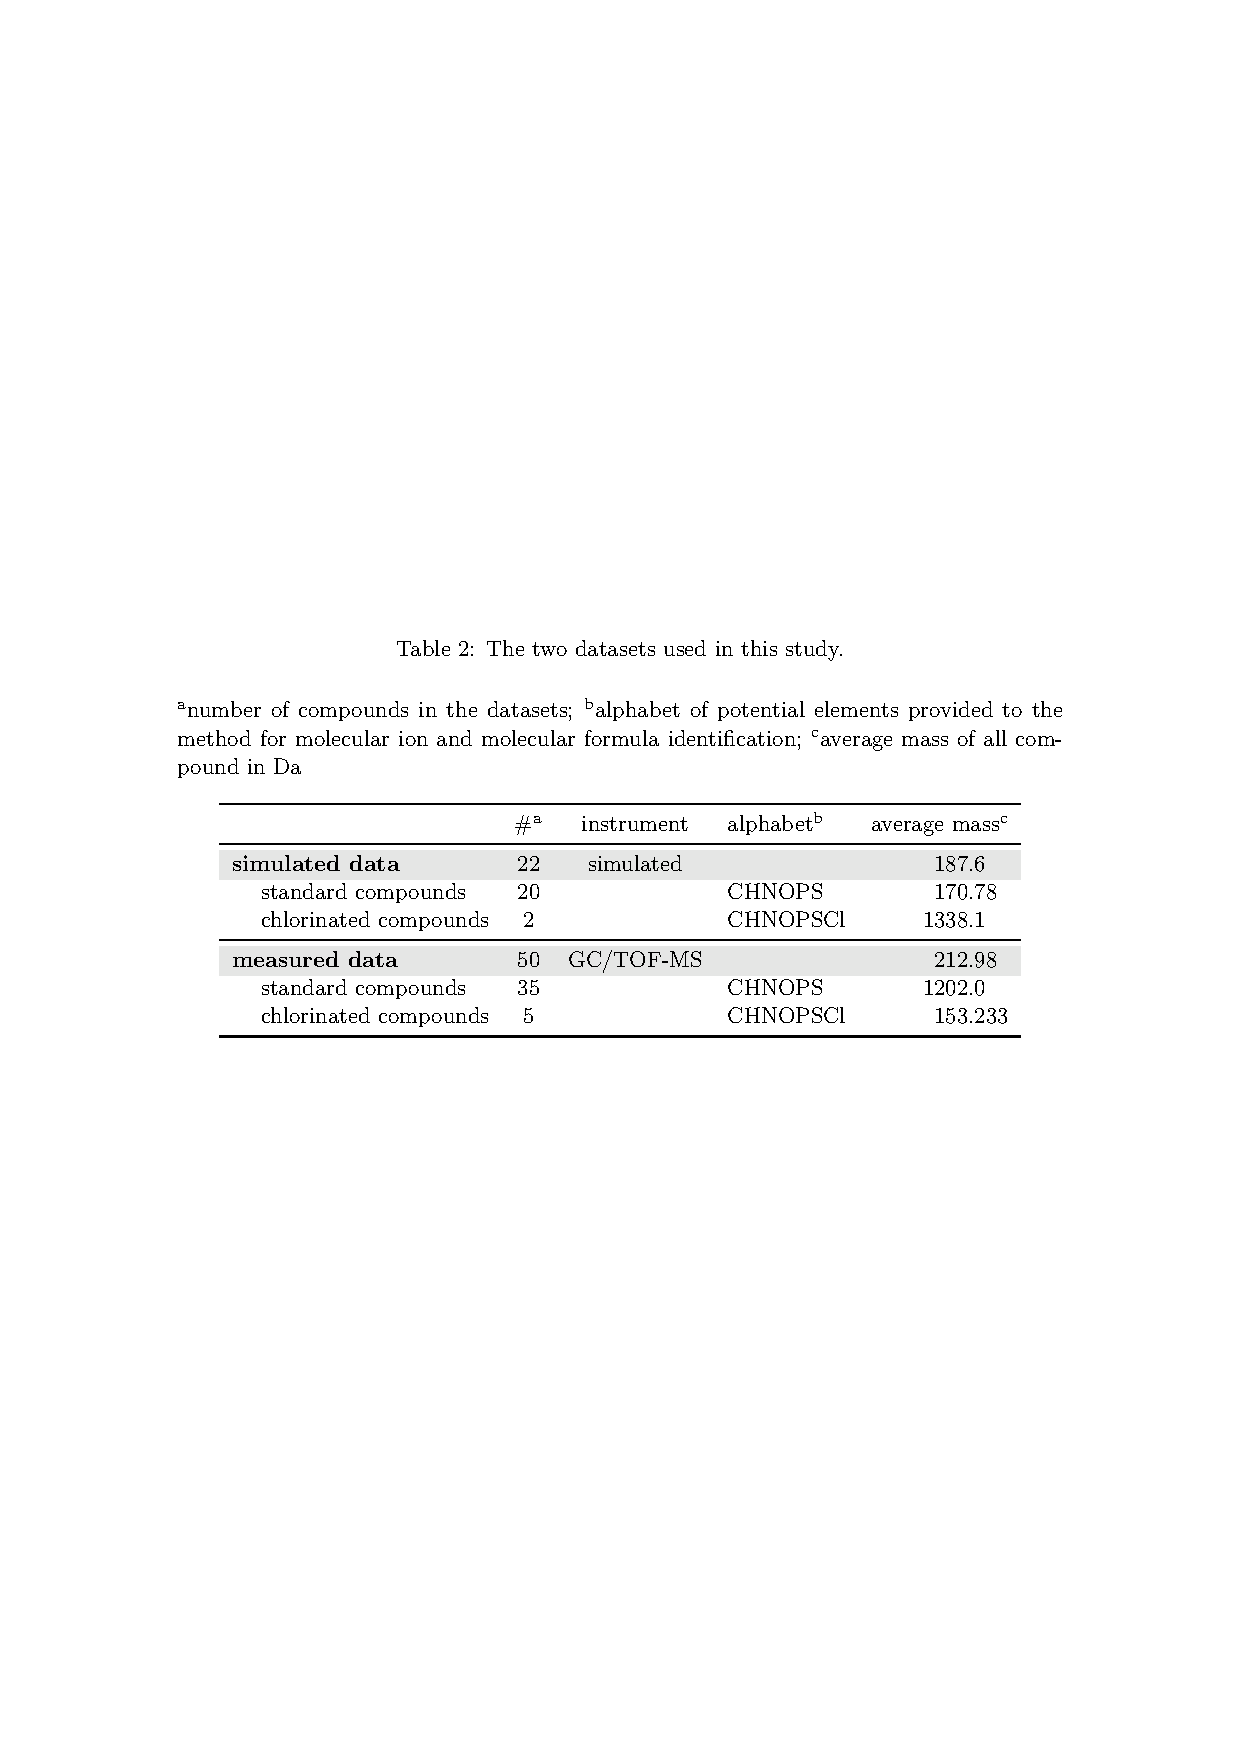
\includegraphics[width=\textwidth]{aufgabe32}
\\
\noindent \underline{nachge\TeX t:}\\
\indent
\begin{table}
\selectlanguage{english}
\caption{The two datasets used in this study.}
\caption*{
\textsuperscript{a}\hspace{-1mm} number of compounds in the datasets; 
\textsuperscript{b}\hspace{-1mm} alphabet of potential elements provided 
				 to the method for molecular ion and molecular formula identification; 
\textsuperscript{c}\hspace{-1mm} average mass of all com- \-pound in Da 
}
\hspace*{0.48cm}
\begin{tabularx}{0.91\textwidth}{llcle{2}}
 \toprule 
				       & \#\textsuperscript{a} 
				       & instrument 
				       & alphabet\textsuperscript{b} 
				       & \textrm{average mass}\textsuperscript{c}\\
 \midrule
 \rowcolor{LessLightGrey}
 \textbf{simulated data} 	       & 22	    & simulated  &              &  187.6\\
 \hspace{0.41cm} standard compounds    & 20	    & 		 & CHNOPS	& 170.78\\
 \hspace{0.41cm} chlorinated compounds & 35	    &            & CHNOPSCl     & 1338.1\\
 \midrule
 \rowcolor{LessLightGrey}
 \textbf{measured data}	       	       & 50         & GC/TOF-MS  & 		& 212.98\\
 \hspace{0.41cm} standard compounds    & 35         & 		 & CHNOPS	& 1202.0\\
 \hspace{0.41cm} chlorinated compounds & 5	    &            & CHNOPSCl     & 153.233\\
 \bottomrule 
  \end{tabularx}
\end{table}

\pagebreak
\begin{aufgabe}
F\"ugen Sie dem Dokument ein Tabellenverzeichnis hinzu. Abbildungs- und Tabellenverzeichnis sollen gemeinsam auf einer eigenen Seite stehen. Die Tabellenunterschriften im Tabellenverzeichnis sollen nicht \"uber eine Zeile hinaus gehen.	
\end{aufgabe}


\pagebreak
\section{Mathematik}					% aufgabe 6
\label{sec:mathematik}
\singlespacing

\begin{aufgabe}\label{aufg:formulas}
\TeX en Sie den Text aus \texttt{aufgabe\ref{aufg:formulas}.pdf} so exakt wie m\"oglich nach.	
\end{aufgabe}

\setlength\parindent{18pt} Wenn A und B beliebige Ereignisse sind und $P(B) \leq 0$ ist, dann ist die bedingte Wahrscheinlichkeit von $A$,
vorausgesetzt $B$ (auch die Wahrscheinlichkeit von $A$ unter der Bedingung $B$, notiert als $P(A \mid B)$, definiert
durch:
\begin{displaymath}
 P(A \mid B) = \frac{P(A \cap B)}{P(B)}
\end{displaymath}
Darin ist $P(A \cap B)$ die Wahrscheinlichkeit, dass $A$ und $B$ gemeinsam auftreten. 
$P(A \cap B)$ wird gemeinsame Wahrscheinlichkeit, Verbundwahrscheinlichkeit oder Schnittwahrscheinlicheit genannt.

\newtheorem{mfze}{Theorem}

%\numberwithin{equation}{}
\begin{mfze}{\textbf{Multiplikationssatz für zwei Ereignisse:}}
\begin{equation}
 P(A \cap B) = P(A \mid B) \cdot P(B)
\end{equation}
\end{mfze}

Verallgemeinert man den obigen Ausdruck des Multiplikationssatzes, der für zwei Ereignisse gilt, erhält man den
allgemeinen Multiplikationssatz. Man betrachte dazu den Fall mit $n$ Zufallsereignissen $A_1$ , $A_2$ , $\ldots$ , $A_n$.

\vspace{0.5cm}
\noindent
\begin{equation*}
 \begin{array}{ccccccccc} 
  P\biggl( \bigcap\limits_{i=1}^{n} A_i \biggl) &
  = &
  P(A_1) &
  \cdot &
  \frac{P(A_1 \cap A_2)}{P(A_1)} &
  \cdot &
  \frac{P(A_1 \cap A_2 \cap A_3)}{P(A_1 \cap A_2)} &
  \cdots &
  \frac{P(A_1 \cap A_2 \cap \cdots \cap A_n)}{ P(A_1 \cap A_2) \cap \cdots \cap A_{n-1}) }\\
    &
   = &
   P(A_1) &
   \cdot &
   P(A_2 \mid A_1) &
   \cdot &
   P(A_3 \mid A_1) \cap A_2) &
   \cdots &
   P\Bigl( A_n | \cap_{i=1}^{n-1} A_i \Bigl) \\
 \end{array}
\end{equation*}

\setlength\parindent{18pt} Sind nur bedingte Wahrscheinlichkeiten und die Wahrscheinlichkeiten des bedingenden
Ereignisses bekannt, ergibt sich die totale Wahrscheinlichkeit von A aus

\begin{mfze}{\textbf{Gesetz der totalen Wahrscheinlichkeit:}}
\begin{equation}
 P(A) = P(A \mid B) \cdot P(B) + P(A \mid B^c) \cdot P(B^c),
\end{equation}
\end{mfze}
\noindent \textit{wobei $B^c$ das Gegenereignis zu $B$ bezeichnet.}\\
\\
\indent Wenn $A$ und $B$ stochastisch unabhängig sind, gilt:
\begin{equation*}
 P(A \cap B) = P(A) \cdot P(B),
\end{equation*}
was dann zu Folgendem führt:

\begin{mfze}{\textbf{Stochastische Unabhängigkeit:}}
\\
\textit{Egal, ob das Ereignis $B$ stattgefunden oder nicht stattgefunden hat, ist die Wahrscheinlich-
keit des Ereignisses $A$ stets dieselbe.}
\\
\begin{equation}
\begin{array}{cccclc}
  P(A \mid B) & = & \frac{P(A) \cdot P(B)}{P(B)}  & = & P(A) & \textit{bzw.} \\
  & & &  = &  P(A \mid B^c) & \\
\end{array}
\end{equation}
\end{mfze}

Für den Zusammenhang zwischen $P(A \mid B)$ und $P(B \mid A)$ ergibt sich direkt aus der
Definition und dem Multiplikationssatz:

\newtheorem{cor}[mfze]{Korollar}
\begin{cor}{\textbf{Der Satz von Bayes:}}
 \begin{equation}
  P(A \mid B) = \frac{P(B \mid A) \cdot P(A)}{P(B)}.
 \end{equation}

\noindent \textit{Dabei kann $P(B)$ im Nenner mit Hilfe des Gesetzes der totalen Wahrscheinlichkeit berechnet werden.}
\end{cor}


\begin{aufgabe}
\TeX en Sie folgende Matrix:
\end{aufgabe}

\noindent \underline{Ursprung:} \\
\hspace{1cm} 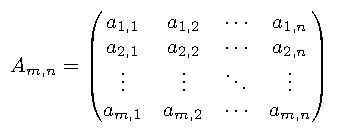
\includegraphics[width=0.4\textwidth]{aufgabe35}

\noindent \underline{nachge\TeX t:}\\ \vspace*{10cm} 
\begin{math}
 \textit{A}_{m,n} =
 \begin{pmatrix}
  a_{1,1} & a_{1,2} & \cdots & a_{1,n}\\
  a_{2,1} & a_{2,2} & \cdots & a_{2,n}\\
  \vdots  & \vdots  & \ddots & \vdots \\
  a_{m,1} & a_{m,2} & \cdots & a_{m,n}\\
 \end{pmatrix}
\end{math}


\pagebreak
\section{Informatik}					% aufgabe 6
\label{sec:informatik}
\subsection{Pseudocode}							% aufgabe 6
\begin{aufgabe}
\TeX en Sie folgenden Pseudocode so exakt wie m\"oglich nach.\\

\noindent \underline{Ursprung:} \\
\noindent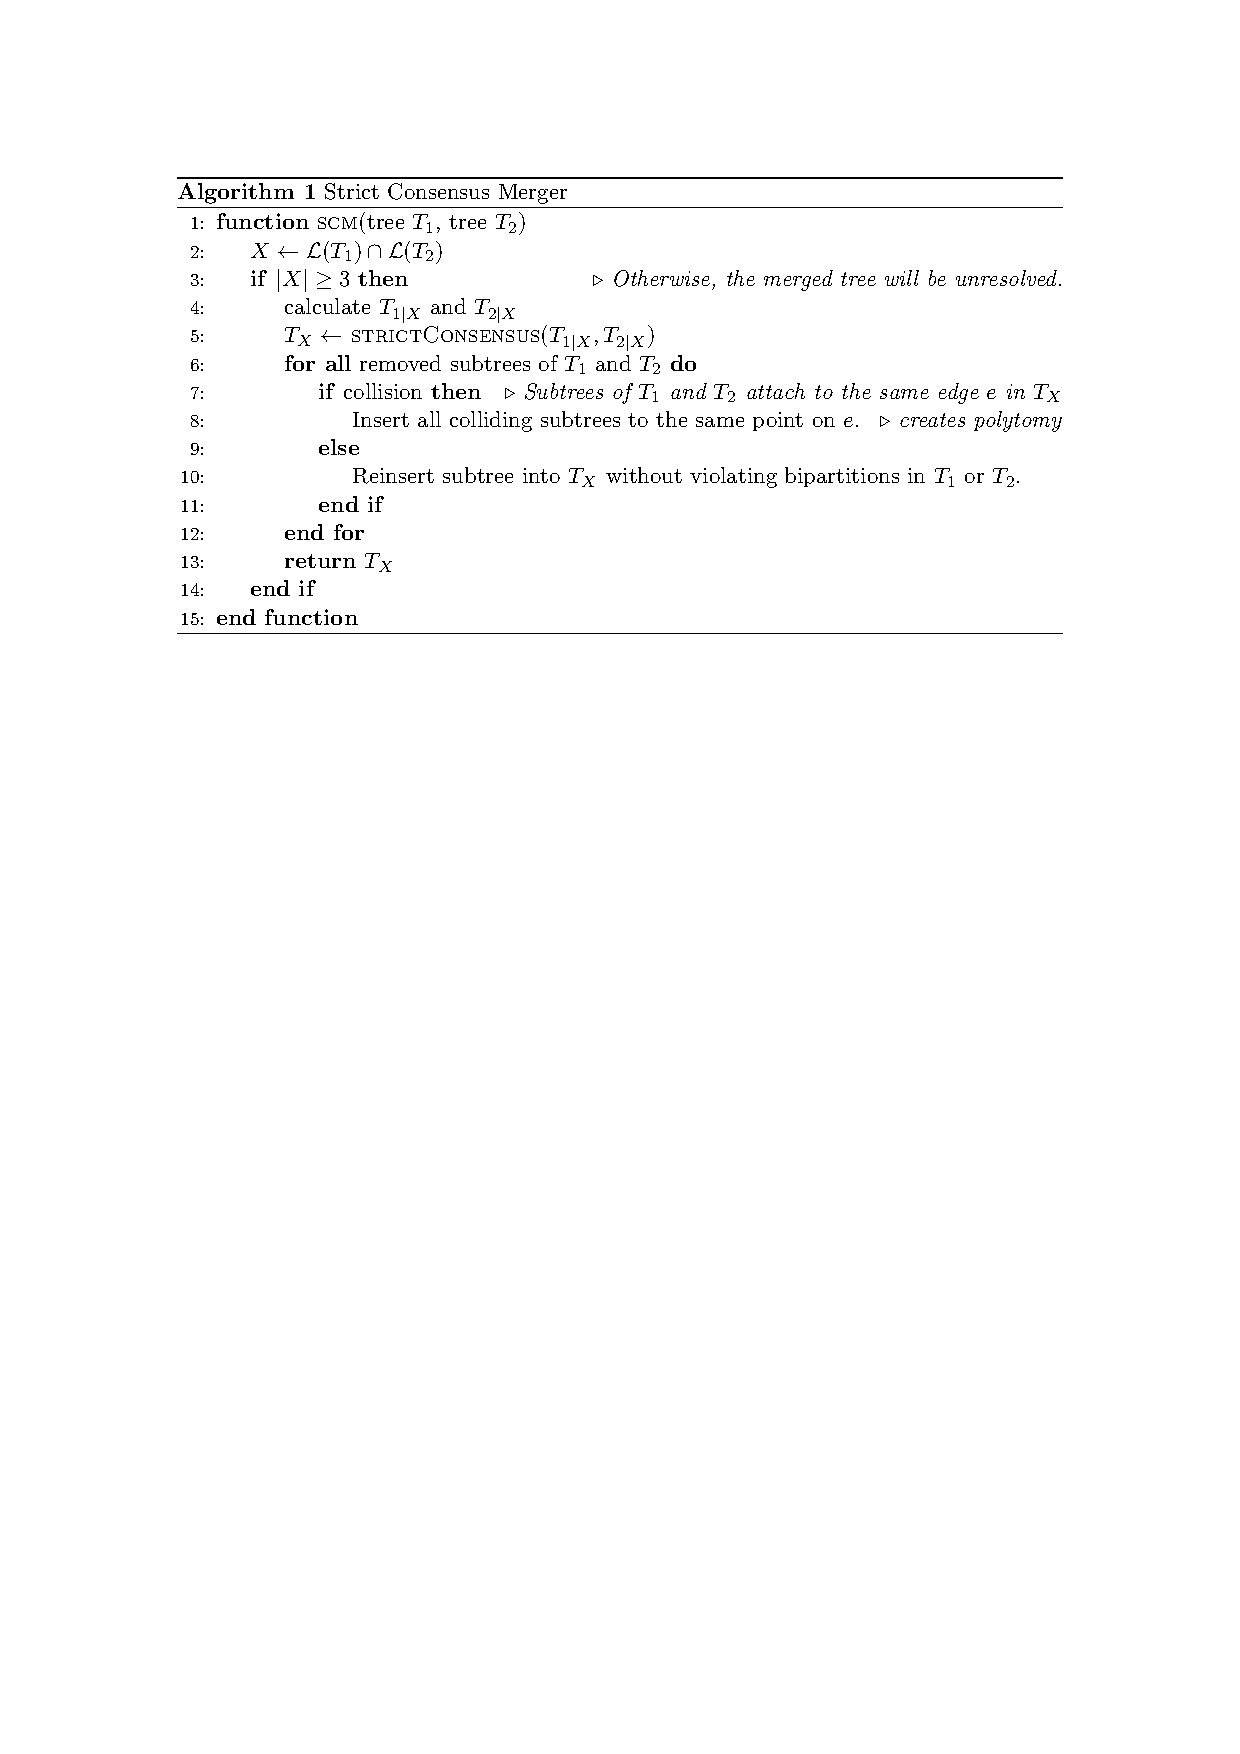
\includegraphics[width=\textwidth]{aufgabe36}	

\noindent \underline{nachge\TeX t:}\\
\begin{algorithm}
   \caption{Strict Consensus Merger}
    \begin{algorithmic}[1]
      \Function{scm}{tree $T_1$, tree $T_2$}
	\State $X \leftarrow \mathcal{L}(T_1) \cap \mathcal{L}(T_2)$
        \If {$|X| \geq 3$}	\Comment{\textit{Otherwise, the merged tree will be unresolved.}}
        \State calculate $T_{1|X}$ and $T_{2|X}$
        \State $T_X \leftarrow$ \Call{strictconsensus}{$T_{1|X},T_{2|X}$}
        \ForAll{removed subtrees of $T_1$ and $T_2$}
	  \If{collision}	\Comment{\textit{Subtrees of $T_1$ and $T_2$ attach to the same edge e in $T_X$}}
	    \State{Insert all colliding subtrees to the same point on $e$.}   \Comment{\textit{creates polytomy}}
	  \Else
	    \State{Reinsert subtree into $T_X$ without violating bipartitions in $T_1$ or $T_2$.}
	  \EndIf
	  \EndFor \\
	\ \  \  \ \ \ \ \ \ \Return{$T_X$}
	\EndIf
       \EndFunction
\end{algorithmic}
\end{algorithm}

\end{aufgabe}

\pagebreak
\subsection{Sourcecode}							% aufgabe 6
\begin{aufgabe}\label{aufg:sourceCode}
\TeX en Sie den Quelltext aus \texttt{aufgabe\ref{aufg:sourceCode}.pdf} so exakt wie m\"oglich nach.(Quelltext: \texttt{AbstractSCMAlgorithm.java})\\ 
\end{aufgabe}

\lstset{ 
  backgroundcolor=\color{white},
  basicstyle=\footnotesize\ttfamily,
  breakatwhitespace=false,
  breaklines=true,
  captionpos=b,
  commentstyle=\color{mygreen},
  deletekeywords={...},
  escapeinside={\%*}{*)},
  extendedchars=true,
  frame=single,
  keepspaces=true,
  keywordstyle=\color{myred},
  language=Java,
  morekeywords={*,...},
  numbers=left,
  numbersep=5pt,
  numberstyle=\tiny\color{mygray},
  rulecolor=\color{white},
  showspaces=false,
  showstringspaces=false,
  showtabs=false,
  stepnumber=1,
  stringstyle=\color{mygray},
  tabsize=4,
  title=\lstname,
  emph={@Override},
  emphstyle={\color{mygold}}
}

\lstinputlisting[language=java]{src/AbstractSCMAlgorithm.java}

\pagebreak
\section{Abschlussarbeiten}				% aufgabe 6
\label{sec:abschlussarbeiten}
\subsection{Große Projekte verwalten und Buchstruktur}				% aufgabe 6
\begin{aufgabe}
Erstellen Sie das Grundger\"ust f\"ur eine eigene Abschlussarbeit. \TeX en
Sie daf\"ur das Layout der Beipsieldatei \texttt{book.pdf} so exakt wie
m\"oglich nach. Auf den Inhalt wird dabei keinen Wert gelegt (verwenden Sie
\texttt{Lorem Ipsum} Text), jedoch auf Titelseite, Kopf-/Fu\ss zeilen,
Seitenzahlen, Abbildung mit Verweis etc. Die Kapitel sollen als einzelne
Dateien vorliegen. Die weiteren Aufgaben dieser Section bearbeiten Sie bitte
an der erstellten Abschlussarbeit. 
\end{aufgabe}

\begin{aufgabe}
F\"ugen Sie der Abschlussarbeit im Anhang eine beliebige Seite aus Ihrem Protokoll hinzu. 
\end{aufgabe}

\begin{aufgabe}
Erm\"oglichen Sie es im Inhaltsverzeichnis per Link zu den jeweiligen Sections zu gelangen. Die Links sollen dabei einen dunklen Blauton haben.  
\end{aufgabe}

\subsection{Hyperlinks und Metadaten}						% aufgabe 6
\begin{aufgabe}
F\"ugen Sie der Abschlussarbeit Metadaten zu Ihrer Person hinzu.
\end{aufgabe}

\begin{aufgabe}
Stellen Sie das Dokument so ein, dass beim \"Offnen das Inhaltsverzeichnis als Lesezeichen angezeigt wird. Die Seiten sollen Seite f\"ur Seite (kein kontinuierliches Scrollen) angezeigt werden. 	
\end{aufgabe}

\subsection{Literaturverzeichnis}						% aufgabe 6
\begin{aufgabe}
Erstellen Sie eine Literaturdatenbank im \texttt{bib} Format mittels
\texttt{JabRef}. F\"ugen Sie mindestens ein Paper (z.B.\ \"uber PubMed), ein
Buch, sowie eine Ver\"offentlichung in einem Konferenzband (z.B.\ LNCS)
hinzu. Verwenden Sie Keys der Form \texttt{autor:YY}. Zitieren Sie alle
Dokumente Ihrer Literaturdatenbank in der Abschlussarbeit im Harvard Stil. Zitieren Sie das
Buch mit Verweis auf eine Seite. Zitate im Text sollen in runden Klammern
stehen. Zitate im Verzeichnis sollen folgendes Format haben:

\medskip
\noindent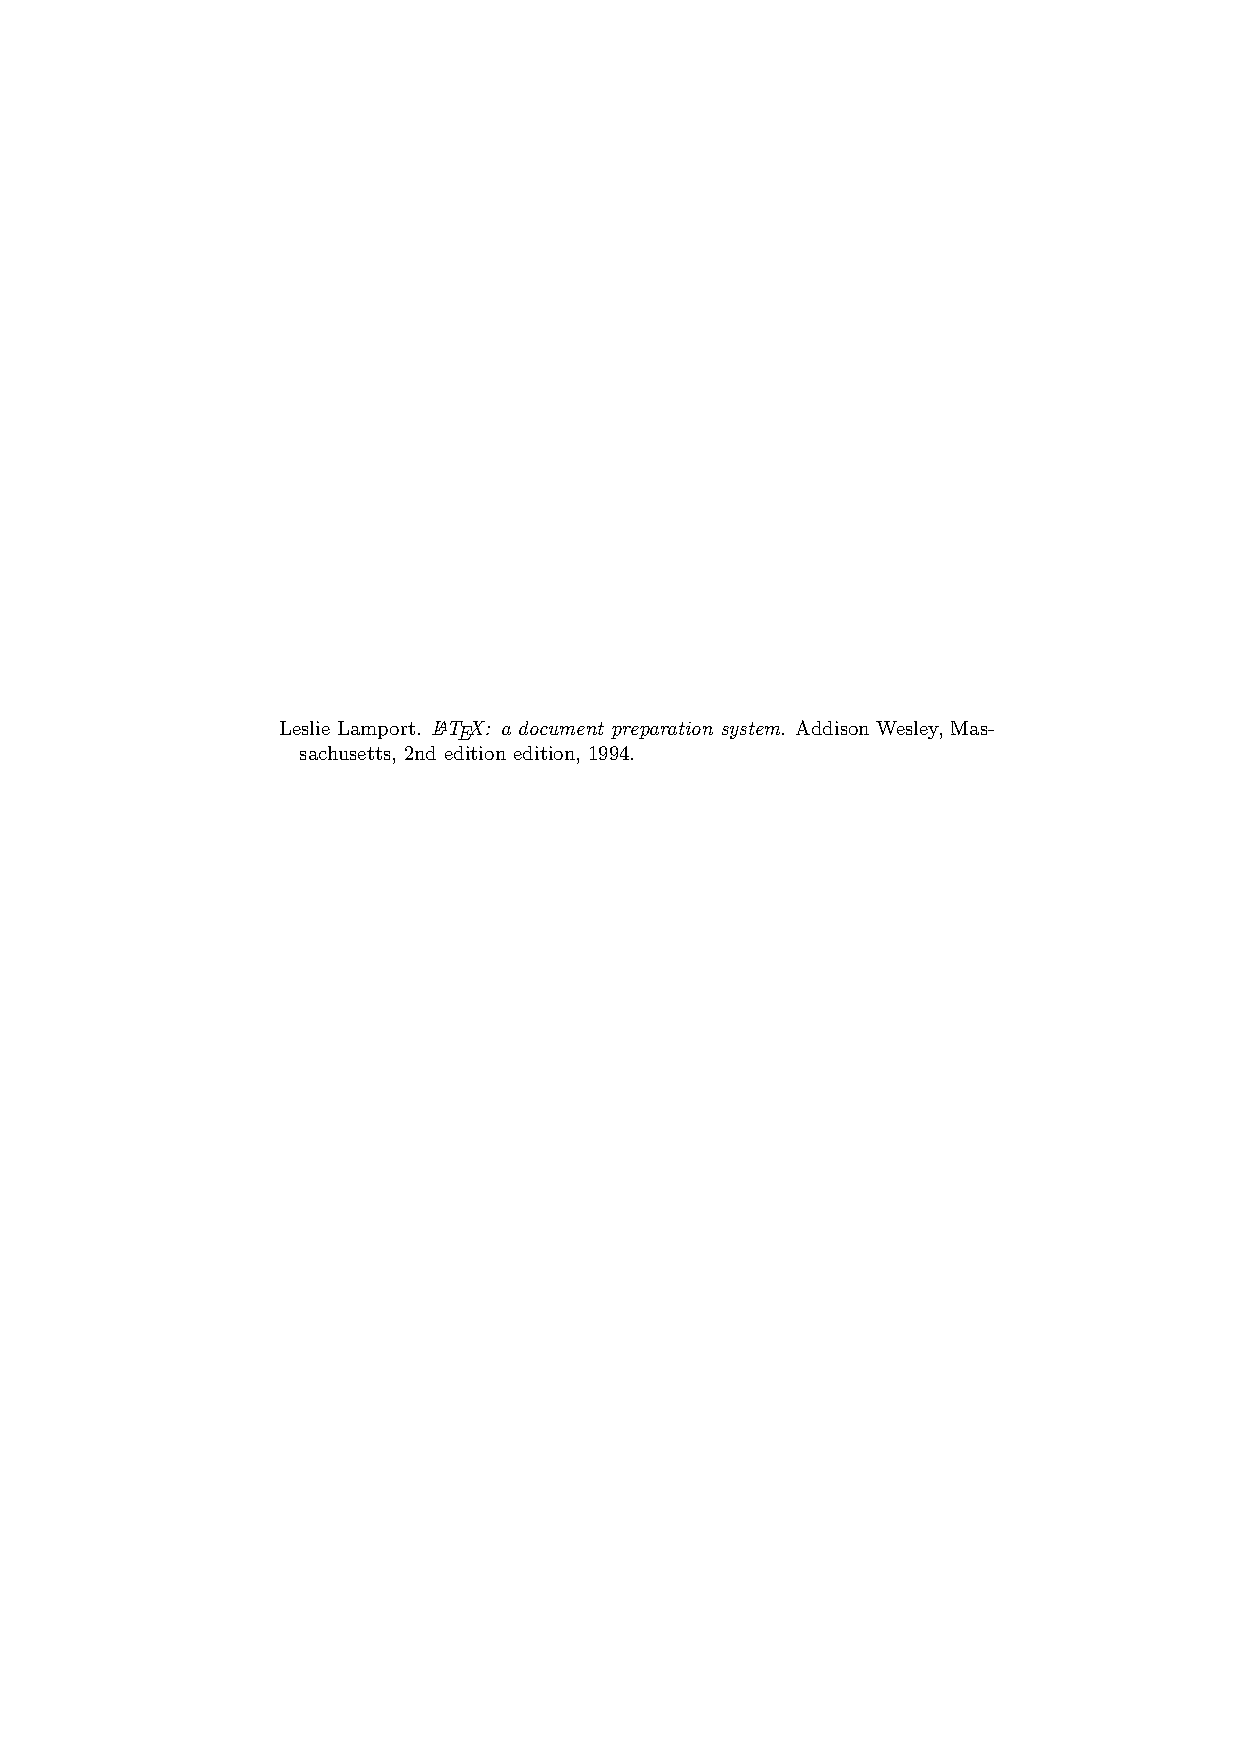
\includegraphics[width=\textwidth]{Literatur}
\end{aufgabe}


\pagebreak
\section{Naturwissenschaftliche Publikationsformate}	% aufgabe 6
\begin{aufgabe}
Erstellen Sie ein eigenes Paper auf Grundlage eines Templates\\
(\texttt{https://www.sharelatex.com/templates/journals}). Denken Sie sich
eine sinnvolle Gliederung aus und f\"ullen Sie inhaltlich alle Stellen die
m\"oglich sind. F\"ur den Rest verwenden Sie wieder \texttt{Lorem Ipsum}
Text. F\"ugen Sie dem Paper ein Literaturverzeichnis hinzu (die bereits
erstellte Literaturdatenbank kann hier wiederverwendet werden).
\end{aufgabe}

\begin{aufgabe}
Erstellen Sie einen Lebenslauf auf deutsch. W\"ahlen Sie ein Template, dass
Ihnen selbst gef\"allt
(\texttt{https://www.sharelatex.com/templates/cv-or-resume}). F\"ullen Sie die
Lebenslauf mit fiktiven Informationen oder f\"ugen Sie, wenn Sie m\"ochten,
ihre eigenen Informationen ein.

\end{aufgabe}

\begin{aufgabe}
Erstellen Sie einen Brief auf Grundlage der \texttt{g-brief} Klasse. Der
Brief soll als Deckblatt f\"ur das komplette Protokoll dienen und eine
Auflistung aller Anh\"ange enthalten. Relevante Informationen (Name,
Matrikelnummer, Mailadresse, Datum, Anschrift) sollen ausgef\"ullt sein;
alle weiteren Informationen k\"onnen ausgedacht oder weggelassen werden.
\end{aufgabe}

\pagebreak
\listoffigures				% aufgabe 27
\listoftables				% aufgabe 33

\label{LastPage}
\end{document}